\documentclass[UTF8,12pt,a4paper]{ctexart}
\usepackage{amsmath,amssymb,amsthm,bm,booktabs,longtable,array,multirow}
\usepackage{geometry,graphicx,float,caption,xcolor,enumitem}
\usepackage[hidelinks]{hyperref}
\geometry{left=2.5cm,right=2.5cm,top=2.5cm,bottom=2.5cm}
\setlength{\parindent}{2em}\setlength{\parskip}{0.10em}
\setlength{\emergencystretch}{3em}
\renewcommand{\baselinestretch}{1.25}
\renewcommand{\topfraction}{0.90}
\renewcommand{\bottomfraction}{0.80}
\renewcommand{\textfraction}{0.08}
\renewcommand{\floatpagefraction}{0.75}
\setcounter{topnumber}{4}
\setcounter{bottomnumber}{2}
\setcounter{totalnumber}{6}
\captionsetup[table]{position=above,font=small}
\setlist{nosep,leftmargin=2em}
\newcommand{\keywords}[1]{\par\noindent\textbf{关键词：}#1}
\newtheorem{proposition}{命题}[section]
\theoremstyle{remark}
\newtheorem*{remark}{说明}
\newcommand{\figslot}[4][3.2cm]{\begin{center}\refstepcounter{figure}
\fbox{\parbox[c][#1][c]{0.88\textwidth}{\centering\small #2}}\par
\small 图~\thefigure\quad #3\label{#4}\end{center}}

\title{考虑预测误差与日内调整的微网购电优化策略}
\author{}\date{}
\begin{document}
\maketitle

\begin{abstract}
针对负荷、光伏和外网电价依次引入不确定性的微网购电问题，本文建立“数据校核—历史数据预测—风险修正—购电计划—滚动调度—费用结算—稳健性检验”的统一框架。全文将计算过程分为购电计划、实际调度和费用结算三个环节，并以决策时可用信息集$\mathcal I_{d,t}$统一四问。每个时刻的决策只使用当时已经获得的信息，实测负荷、实际光伏发电量和实际电价不提前参与决策。

针对问题一，建立含日末状态回归约束的确定性线性规划。求得典型日全天计划购电量为$59482.70\ \mathrm{kWh}$，购电费用为$35126.95$元。储能电量始终位于$1200$至$10800\ \mathrm{kWh}$，且日初、日末均为$6000\ \mathrm{kWh}$，说明所得调度既利用峰谷价差，又没有透支次日储能。

针对问题二，比较两种仅使用历史数据的预测方法。F1用7天前同一时段的负荷和前7天同一时段的平均光伏，F2将7、14、21天前同一时段的负荷取中位数，光伏预测仍采用前7天平均值。本文采用F1，并依据5倍应急价格与计划电价的比值推出风险裕量的理论分位$0.8$，再由历史残差经验分位数实现；本文以$W=35,\alpha=0.805,H=49$作为主方案固定参数进行全年模拟，总费用为$14786101.35$元，应急购电量为$245483.29\ \mathrm{kWh}$。

针对问题三，按0:00、6:00、12:00和18:00四个预报时点更新购电计划，并规定每个时段的最终购电量只相对0:00原计划结算一次。以$W=35,\alpha=0.7725,H=6$作为主方案固定参数进行全年逐日模拟，所得总费用为$14664345.40$元。八种预报使用方案的样本内费用比较表明，使用全部日内预报相对不使用日内新预报减少$566030.72$元，平均盈亏平衡更新成本为$564.90$元/次。

针对问题四，利用历史信息预测电价以制定购电计划，并按附件4的实际电价结算。采用近30日中位数预测电价时，固定购电计划与可调整购电计划的费用分别为$17378687.69$元和$15465962.60$元；允许三次调整后样本内费用减少$1912725.09$元，并将应急购电量由$570732.66\ \mathrm{kWh}$降至$210394.02\ \mathrm{kWh}$。与“事后理想信息基准”（即假设0:00已知全天实际电价、仅用于事后对照而不参与实际决策的理想情形）相比，两种模式的样本内费用差异分别为$78602.31$元和$82912.80$元。

全年逐日模拟中供需平衡、SOC递推和费用汇总均通过数值校验，全部物理约束满足。预报组合对比、样本内费用差异和$\kappa^*$定量比较了不同预报时点的影响；尾部风险检验进一步表明，可调整购电计划同时降低平均费用和极端高费用情况下的损失。
\keywords{微网购电；线性规划；分位风险修正；滚动优化；样本内费用比较}
\end{abstract}
\clearpage

\section{问题重述}
某并网型微网由小区负荷、光伏发电、储能设备和外部电网组成。外网购电既要保证供能不低于负荷，又要利用储能完成低价充电和高价放电。题目按信息条件逐步增加难度：问题一给定典型日数据；问题二引入全年负荷和光伏波动及5倍价格的紧急购电；问题三允许在0:00、6:00、12:00和18:00依据新光伏预报调整合同；问题四再引入实时波动电价。本文分别给出各问的模型、结果和比较分析。

储能额定容量为$12000\ \mathrm{kWh}$，运行电量限制在$1200$至$10800\ \mathrm{kWh}$，最大充放电功率为$5000\ \mathrm{kW}$，充放电效率均取0.9。2025年1月1日0:00的储电量为$6000\ \mathrm{kWh}$，每日划分为144个10分钟时段。

四问最终都要求输出逐时段购电、充放电和应急购电结果，但决策权限不同。问题一回答确定数据下的调度；问题二处理日前计划与实测负荷、光伏之间的偏差及其应急成本；问题三利用日内新版光伏预报调整尚未执行的合同；问题四在价格未知时比较固定合同和可调合同。模型因此需要同时明确决策时可用的信息、合同生效时间和费用结算口径。

\section{问题分析}
四问共享同一物理系统，但决策时可获得的信息和结算规则不同。若把所有变量放入一个优化模型，容易把尚未观测的负荷、光伏或电价误当成已知量。本文将计算过程分为购电计划、实际调度和费用结算三个环节：购电计划只使用当时可获得的信息；实际调度根据购电计划、预测结果和当前储能状态确定当前时段的调度决策；获得实测数据后再修正调度并计算费用。由此严格区分计划购电量、调整购电量和实际有效供能。

问题一是确定性线性规划。问题二的难点是预测误差与5倍应急价格之间的权衡，因此比较F1、F2后，根据净负荷历史残差的分位数加入风险裕量。问题三必须使预报发布时间、购电调整生效时间、实际SOC和结算基准严格对齐。问题四还需区分预测电价与实际结算电价，不能把附件4的全年实际电价当作0:00已知信息。全文技术路线见图\ref{fig:route}。

本文严格区分在线决策与事后评价。在线决策仅使用决策时刻之前已经获得的历史观测、当前储能状态、已生效合同及已发布预测；当天未来的实际负荷、实际光伏和实际电价不进入该时刻的决策。所有真实运行数据仅在对应时段决策形成后用于执行修正、费用结算和统计评价。正式模拟过程中，主方案参数保持固定，不根据未来实际运行结果在线更新。若参数曾通过同一年度样本回放比较确定，则相关年度指标仅解释为样本内闭环回放结果，不代表严格的外样本无偏性能。
\begin{figure}[htbp]\centering

\includegraphics[width=0.88\textwidth]{figures/route.png}
\caption{全文技术路线图}\label{fig:route}\end{figure}

图\ref{fig:route}将购电计划优化与实际调度分开。前者决定需要购买多少电，后者决定已购电、光伏和储能怎样共同满足实测负荷；若二者混为一谈，就会把最终实际购电量误作日前计划，也无法正确计算弃购和应急费用。问题一在确定性线性规划处结束，问题二从预测和风险修正处接入，问题三增加日内购电调整环节，问题四再把固定电价替换为基于历史信息的电价预测。这样四问共享一套物理约束，差异只来自决策时可用信息和结算规则，便于在相同条件下比较。

\subsection{四问的差异与统一求解}
四问共享同一储能和供需平衡约束，差异来自信息和结算条件：问题一处理确定性日前调度；问题二在预测误差和5倍应急价格下确定日前购电计划；问题三利用日内光伏预报调整尚未执行的购电量；问题四同时处理光伏与电价的不确定性。比较这些方案时，预测来源、调度方法和结算口径保持一致。

本文采用连续线性规划表达供需平衡、SOC递推、购电量调整和分段费用；微网能量管理中的优化建模方法可参见综述\cite{nemati2018unitcommitment,thirunavukkarasu2022optimization}。在非负电价和效率损失下，同时充放电不会改善目标，模拟结果也验证了这一点。历史残差通过经验分位数转化为风险裕量，逐步获得的信息通过滚动优化处理：每次规划未来若干时段，只执行当前时段的决策，再将时段结束时的实际SOC传入下一时段。该求解方式保留了储能跨时段约束，并在所定义的信息访问规则下不调用未来实测数据。

这里的“因果”仅针对逐日运行过程：每个时段的执行决策只使用当时已经获得的观测、合同和预报。$W$、$\alpha$和$H$等全局参数由给定年度样本的闭环回测确定，因此本文年度结果属于该样本内的策略评价；它不等同于对未知年份的无偏外样本检验。

\section{数据处理与特征分析}
\subsection{数据结构与时间对齐}
附件1含144个典型日电价、负荷和光伏预测点；附件2和附件4连续覆盖2025年365天，每天144个点；附件3每天在四个时刻发布未来24小时整点光伏预报。原始负荷和光伏为kW，进入模型前换算为
\begin{equation}E_t=P_t\Delta t,\qquad \Delta t=\frac{1}{6}\ \mathrm{h}.\label{eq:power-energy}\end{equation}
因此单个时段最大充放电量为$B_{\max}=5000/6=833.3333\ \mathrm{kWh}$。原始时间标记从00:10至次日00:00，按时段结束时刻解释；计算按原始行序进行，输出保留题目模板列序。

为防止时间错位，本文以“区间起点作决策、区间终点记录结果”为统一口径。例如原始标签00:10对应$[00{:}00,00{:}10)$，附件3整点预报先按发布时间和目标时刻定位，再插值到10分钟网格。所有年度预测均满足历史日$j<d$，1月只参与残差窗口预热和SOC连续传递，不计入正式费用。缺失值、负负荷、负光伏以及日期重复均在读入阶段检查。

数据处理遵循“原始量不改写、派生量单独保存”的原则。附件2的实测负荷与实际光伏发电量用于模拟计算和事后评价，附件3的多版本光伏预测用于问题三、四的决策输入，附件4的实际电价只用于结算和事后理想信息基准对照。对附件3从整点到10分钟网格的插值只在相邻已发布预测点之间进行，不跨越发布时间调用未来版本；各版本曲线以发布时刻已完成的实测光伏作为插值锚点，再向未来整点预报展开，因此只使用发布时刻已经获得的信息。对于凌晨尚无足够35日历史的情形，使用已有历史构造经验分位；随着预热日增加，窗口自然扩展到设定长度。这样既保留年初可运行性，也保证2月正式窗口使用完整风险样本。

为统一量纲，本文在进入优化器前完成全部功率--电量转换，优化变量一律使用kWh/时段；只有预测误差表和数据特征图保留kW。该区分十分必要：若把$5000\ \mathrm{kW}$直接当成单个时段的充电量，时段能量约束会被放大6倍，导致SOC边界和费用结果同时失真。费用则统一以元为基本单位，正文在比较大额差异时再换算为万元，但不改变底层计算精度。

\subsection{典型日与全年分布}
\begin{figure}[htbp]\centering

\includegraphics[width=0.96\textwidth]{figures/data-overview.png}
\caption{微网典型日与全年负荷、光伏数据全景}\label{fig:data-overview}\end{figure}

图\ref{fig:data-overview}反映了峰谷电价与净负荷的错位，以及负荷和光伏的季节规律。光伏预报误差与提前期的关系直接服务于问题三的风险校正，故将相应诊断图移至问题三模型之后，使数据证据与模型选择相邻呈现。

\section{模型假设与符号说明}
\subsection{模型假设及其作用}
\begin{enumerate}
\item \textbf{外网单向供电。}外购电量非负，不允许向外网售电。题目未给出并网功率上限，故不另设购电上限。该假设决定了购电变量的方向；若实际系统允许反向售电，需增加售电变量、售电价格和并网容量约束。
\item \textbf{允许弃光和弃购。}无法被负荷或储能吸收的光伏可以舍弃且不收取额外罚金；已签合同但未使用的电量不退款。该假设使供需平衡方程在光伏过剩或计划购电量偏大时仍保持可行，并区分“弃光”和“已付费弃购”两种经济含义不同的冗余。
\item \textbf{储能参数在单个时段内恒定。}主模型取$\eta_c=\eta_d=0.9$，充放电功率上限及SOC边界不随时间变化。效率进入状态递推而不是供需平衡方程；针对“0.9为往返效率”的另一解释，后文改取$\eta_c=\eta_d=\sqrt{0.9}$重新计算。
\item \textbf{决策不使用未来信息。}时刻$t$的购电计划或储能调度只能使用已完成观测、当前SOC、当前购电量和截至$t$已发布的预测，不能读取未来的实测负荷、实际光伏发电量或实际电价。该假设是问题二至问题四公平比较的共同前提。
\item \textbf{应急购电只负责保供。}应急电仅填补当前时段计划购电、光伏和可行放电之后的剩余缺口，不用于主动给储能充电。由此，5倍电价对应供电不足的惩罚，而不是一个可供套利的普通能源通道。
\item \textbf{购电调整只在授权时刻生效。}问题三和问题四的可调整方案仅在0:00、6:00、12:00和18:00更新尚未执行的购电量，已执行时段及其已发生费用不再调整。每个目标时段的最终购电量只相对0:00原计划结算一次。
\item \textbf{年度SOC连续传递。}问题二至问题四从2025年1月1日0:00的$6000\ \mathrm{kWh}$开始连续模拟，不强制每日末SOC回到日初；1月用于状态和历史窗口预热，2月1日至12月31日计入正式费用。该处理避免人为制造每日免费复位。
\item \textbf{10分钟离散足以描述调度。}每个时段内的负荷、光伏和电价以区间代表值计算，时段内更高频波动不单独建模。功率先乘$\Delta t=1/6\ \mathrm h$转为电量，因此所有平衡式均以$\mathrm{kWh}$/时段为口径。
\end{enumerate}

八条假设分别对应外网边界、冗余处理、储能物理、决策信息、保供机制、交易权限、跨日状态和离散精度。对效率、初始SOC、容量、功率、误差倍率、时间标记和结算口径的偏离均在后文重新求解或审计；因此，模型结论只在上述条件内成立。

\subsection{索引、集合与参数}
全文以表\ref{tab:index-parameters}和表\ref{tab:variables}统一说明符号。上标$P$表示规划量，上标$E$表示实际执行量；无上标时由上下文确定。功率只在原始数据和预测误差评价中使用$\mathrm{kW}$，进入优化器后一律使用电量。
\begin{table}[htbp]\centering\small\caption{索引、集合与主要参数}\label{tab:index-parameters}
\begin{tabular}{p{0.16\textwidth}p{0.50\textwidth}p{0.24\textwidth}}\toprule 符号&定义&单位或范围\\\midrule
$d,j$&目标日与历史日，预测时必须满足$j<d$&日\\
$t,\tau$&日内10分钟时段索引&$1,\ldots,144$\\
$r,h$&预报发布时刻与提前期&$r\in\{0,6,12,18\}$，$h=1,\ldots,24$ h\\
$\mathcal T_r,\mathcal H_t$&第$r$次预报更新后的剩余时段集合、时刻$t$的滚动时域&集合\\
$\Delta t$&单个时段持续时间&$1/6\ \mathrm h$\\
$S_{\min},S_{\max},S_0$&SOC下界、上界及年初值&1200，10800，6000 kWh\\
$B_{\max}$&单个时段最大充电量或放电量&833.3333 kWh\\
$\eta_c,\eta_d$&充电效率与放电效率&0.9，0.9\\
$W,\alpha,H$&残差窗口、风险分位和滚动时域长度&日、无量纲、时段数\\
$\lambda,\varepsilon$&终端电量价值、充放电辅助惩罚系数&元/kWh，正小数\\\bottomrule
\end{tabular}\end{table}

\subsection{状态、决策与结算变量}
\begin{table}[htbp]\centering\small\caption{状态、决策与结算变量}\label{tab:variables}
\begin{tabular}{p{0.20\textwidth}p{0.52\textwidth}p{0.18\textwidth}}\toprule 符号&定义&单位\\\midrule
$L_t,V_t,N_t$&实测负荷、可用光伏发电量、净负荷$L_t-V_t$&kWh/时段\\
$\widehat L_t,\widehat V_t,\widehat N_t$&基础预测负荷、光伏和净负荷&kWh/时段\\
$\widetilde L_t,\widetilde V_t,\widetilde N_t$&加入风险裕量后修正的负荷、光伏和净负荷预测&kWh/时段\\
$p_t,q_t,g_t$&0:00原计划购电量、最终调整购电量、当前时段生效购电量&kWh/时段\\
$x_t,y_t,S_t$&交流侧充电量、放电量、时段初储电量&kWh/时段，kWh\\
$v_t$&实际被负荷或储能利用的光伏发电量&kWh/时段\\
$u_t,w_t$&紧急购电量、已付费但未利用的计划购电量&kWh/时段\\
$\delta_t^+,\delta_t^-$&相对$p_t$的向上、向下购电调整量&kWh/时段\\
$c_t,\widehat c_t$&实际结算电价、决策时预测电价&元/kWh\\
$e^N_{j,t},R_{d,r,h}$&净负荷历史残差、按提前期设置的风险裕量&kWh/时段\\
$C,\kappa^*$&实际总费用、单次更新盈亏平衡成本&元，元/次\\\bottomrule
\end{tabular}\end{table}

\subsection{统一物理约束与决策时可用信息}
储能状态转移与边界为
\begin{align}
S_{t+1}&=S_t+\eta_cx_t-\frac{y_t}{\eta_d},\label{eq:soc}\\
1200\le S_t&\le10800,\qquad0\le x_t,y_t\le833.3333.\label{eq:battery-bound}
\end{align}
实际调度环节的供需平衡方程为
\begin{equation}g_t-w_t+v_t+y_t+u_t=L_t+x_t,\quad0\le v_t\le V_t,\quad0\le w_t\le g_t.\label{eq:bus-balance}\end{equation}
式\eqref{eq:soc}中，$\eta_cx_t$是实际进入电池的电量，$y_t/\eta_d$是为向交流侧送出$y_t$而消耗的电量；效率只出现一次，避免重复折损。式\eqref{eq:bus-balance}左侧依次为有效计划购电、实际光伏发电量、放电和紧急购电，右侧为负荷与充电，表示供给与用电需求相等。$w_t$从计划购电量中扣除，因此弃购不被误记为实际供能。连续LP在费用目标之后加入减少不必要充放电的辅助惩罚项，以便从多个费用相同的最优方案中选择充放电量较少的方案；该辅助项和终端价值都不计入最终购电费用。

为了统一四问，进一步定义信息集
\begin{equation}
\mathcal I_{d,t}=\{\text{已完成历史观测},\ S_{d,t},\ \text{当前生效合同},\ \text{截至}t\text{已发布预测}\}.
\label{eq:info-set}
\end{equation}
所有购电量更新和当前时段的计划调度均为$\mathcal I_{d,t}$的函数。当前时段的实测负荷和实际光伏发电量只在计划调度形成后用于实测修正、供需平衡和费用结算，因此不使用本时段结束后才得到的数据指导本时段决策。由此，预测模型、滚动调度方法和价格策略可以在相同的决策时序下比较。

\section{问题一：确定性日前购电模型}
\subsection{模型建立}
令$g_t=p_t$，规划层满足
\begin{equation}g_t+v_t+y_t=L_t+x_t,\qquad0\le v_t\le V_t,\label{eq:q1-balance}\end{equation}
并设置$S_1=S_{145}=6000$。目标为
\begin{equation}\min C_1=\sum_{t=1}^{144}c_tg_t.\label{eq:q1-obj}\end{equation}
模型为连续线性规划，使用HiGHS求解器完成计算\cite{virtanen2020scipy}。

模型中允许三条供能路径：光伏直接供负荷或进入储能，外网电直接供负荷或进入储能，储能只能向负荷放电。充电效率作用于SOC增量，放电效率作用于SOC扣减；这种交流侧计量使电网购电、光伏利用量和负荷量保持同一单位，也避免把往返效率重复计算。

式\eqref{eq:q1-balance}表达每个10分钟时段的能量守恒，式\eqref{eq:q1-obj}则只统计实际支付的合同电费。终端条件$S_{145}=S_1$用于固定日末储能资产状态，避免模型在最后一个时段把电池放空来虚降当日费用，从而保证不同方案可在同一状态基准下比较。

\subsection{模型性质与理论校验}
\begin{proposition}[循环SOC下的全天能量恒等式]\label{prop:q1-energy}
若问题一全天无弃光，即$v_t=V_t$，且$S_{145}=S_1$，令$X=\sum_tx_t$、$Y=\sum_ty_t$、$G=\sum_tg_t$，则
\begin{equation}
Y=\eta_c\eta_dX,\qquad
G=\sum_tL_t-\sum_tV_t+(1-\eta_c\eta_d)X.
\label{eq:q1-identity}
\end{equation}
\end{proposition}
\begin{proof}
对式\eqref{eq:soc}在全天求和，左端状态增量为$S_{145}-S_1=0$，故$\eta_cX-Y/\eta_d=0$，得到$Y=\eta_c\eta_dX$。再对式\eqref{eq:q1-balance}求和并代入$v_t=V_t$，有$G+\sum_tV_t+Y=\sum_tL_t+X$；将第一式代入即可得到第二式。
\end{proof}

命题\ref{prop:q1-energy}给出不依赖求解器的独立检查。第一式检验SOC递推和效率位置是否正确；第二式说明购电量等于基础净负荷再加上电池往返损耗。若数值结果不满足该式，通常意味着功率--电量换算、时间索引或效率处理存在错误。

\begin{proposition}[连续LP中可消除的充放电循环]\label{prop:no-cycle}
设$c_t\ge0$，系统不允许售电，也不存在充放电补贴。若某个可行解在时段$t$满足$x_t>0,y_t>0$，且存在
\[
0<\delta\le\min\!\left(x_t,\frac{y_t}{\eta_c\eta_d}\right),\qquad
(1-\eta_c\eta_d)\delta\le g_t+v_t.
\]
则可以在保持SOC增量和供需平衡不变的情况下减少该时段吞吐量，并且购电成本不增加。因此，在费用相同时优先选择充放电量较少的方案，不会保留这类可消除的同时充放电循环。
\end{proposition}
\begin{proof}
令$x'_t=x_t-\delta$、$y'_t=y_t-\eta_c\eta_d\delta$。此时
$\eta_cx'_t-y'_t/\eta_d=\eta_cx_t-y_t/\eta_d$，故SOC增量不变。充电减少量比放电减少量多$(1-\eta_c\eta_d)\delta$，只需从$g_t$和$v_t$中合计减少同样电量，供需平衡仍成立。由于$c_t\ge0$，减少购电不会提高主目标；同时$x'_t+y'_t<x_t+y_t$，故原解不可能是吞吐量最小的同费用解。
\end{proof}

命题\ref{prop:no-cycle}说明本文在非负电价、无售电和无吞吐补贴的题设下可以优先采用连续LP，而无需一开始就引入0--1互斥变量。该命题是充分条件而不是无条件结论；若出现负电价、售电收益或循环补贴，应改用显式互斥MILP。本文全部模拟计算中$\min(x_t,y_t)=0$，与该理论判断一致。

\subsection{求解流程}
首先把附件1的功率序列转为单时段电量，并按价格、负荷、光伏顺序组装目标向量和等式约束；其次联立144个供需平衡方程和145个SOC状态，加入初末状态相等条件；最后调用HiGHS求解连续LP，并以供需平衡残差、SOC递推残差和两条总量恒等式进行复核。问题一为确定性算例，其典型日数据在建模阶段即已给定；由于不存在后续观测带来的新信息，直接求解整日模型即可。

\subsection{求解结果与校验}
全天购电量为$59482.70\ \mathrm{kWh}$，购电费用为$35126.95$元，日初、日末储电量均为$6000\ \mathrm{kWh}$。指定时段结果见表\ref{tab:q1-slots}。
\begin{table}[htbp]\centering\caption{问题一指定时段购电量}\label{tab:q1-slots}
\begin{tabular}{cccccc}\toprule10:00&12:00&14:00&16:00&18:00&20:00\\\midrule
0.00&480.41&0.00&445.43&531.89&0.00\\\bottomrule
\multicolumn{6}{c}{单位：kWh；每列对应其后10分钟时段。}\end{tabular}\end{table}
\begin{table}[htbp]\centering\caption{问题一分时段充放电结果}\label{tab:q1-blocks}
\begin{tabular}{crr}\toprule 时段&充电量/kWh&放电量/kWh\\\midrule
0:00--4:00&4500.00&0.00\\4:00--8:00&833.33&6365.84\\
8:00--12:00&4787.96&1703.00\\12:00--16:00&5286.04&91.10\\
16:00--20:00&0.00&5780.13\\20:00--24:00&5333.33&2859.87\\\bottomrule
\end{tabular}\end{table}
\begin{figure}[htbp]\centering

\includegraphics[width=0.96\textwidth]{figures/q1-operation.png}
\caption{问题一最优购电调度与储能状态轨迹}\label{fig:q1-operation}\end{figure}

图\ref{fig:q1-operation}呈现低价时段充电、高价时段放电的跨时段搬移特征；表\ref{tab:q1-blocks}中同一4小时区间同时出现充、放电，是不同时段汇总所致。SOC取值始终位于$[1200,10800]\ \mathrm{kWh}$。
供需平衡方程和SOC递推均满足逐时段约束，命题\ref{prop:q1-energy}两条全天恒等式的残差均低于$10^{-11}\ \mathrm{kWh}$，由此从逐时段约束和全天总量两个尺度完成交叉校验。

\section{问题二：考虑预测误差的日前购电与滚动调度}
问题二的预测、风险修正与滚动执行关系见图\ref{fig:q2-flow}。
\begin{figure}[htbp]\centering
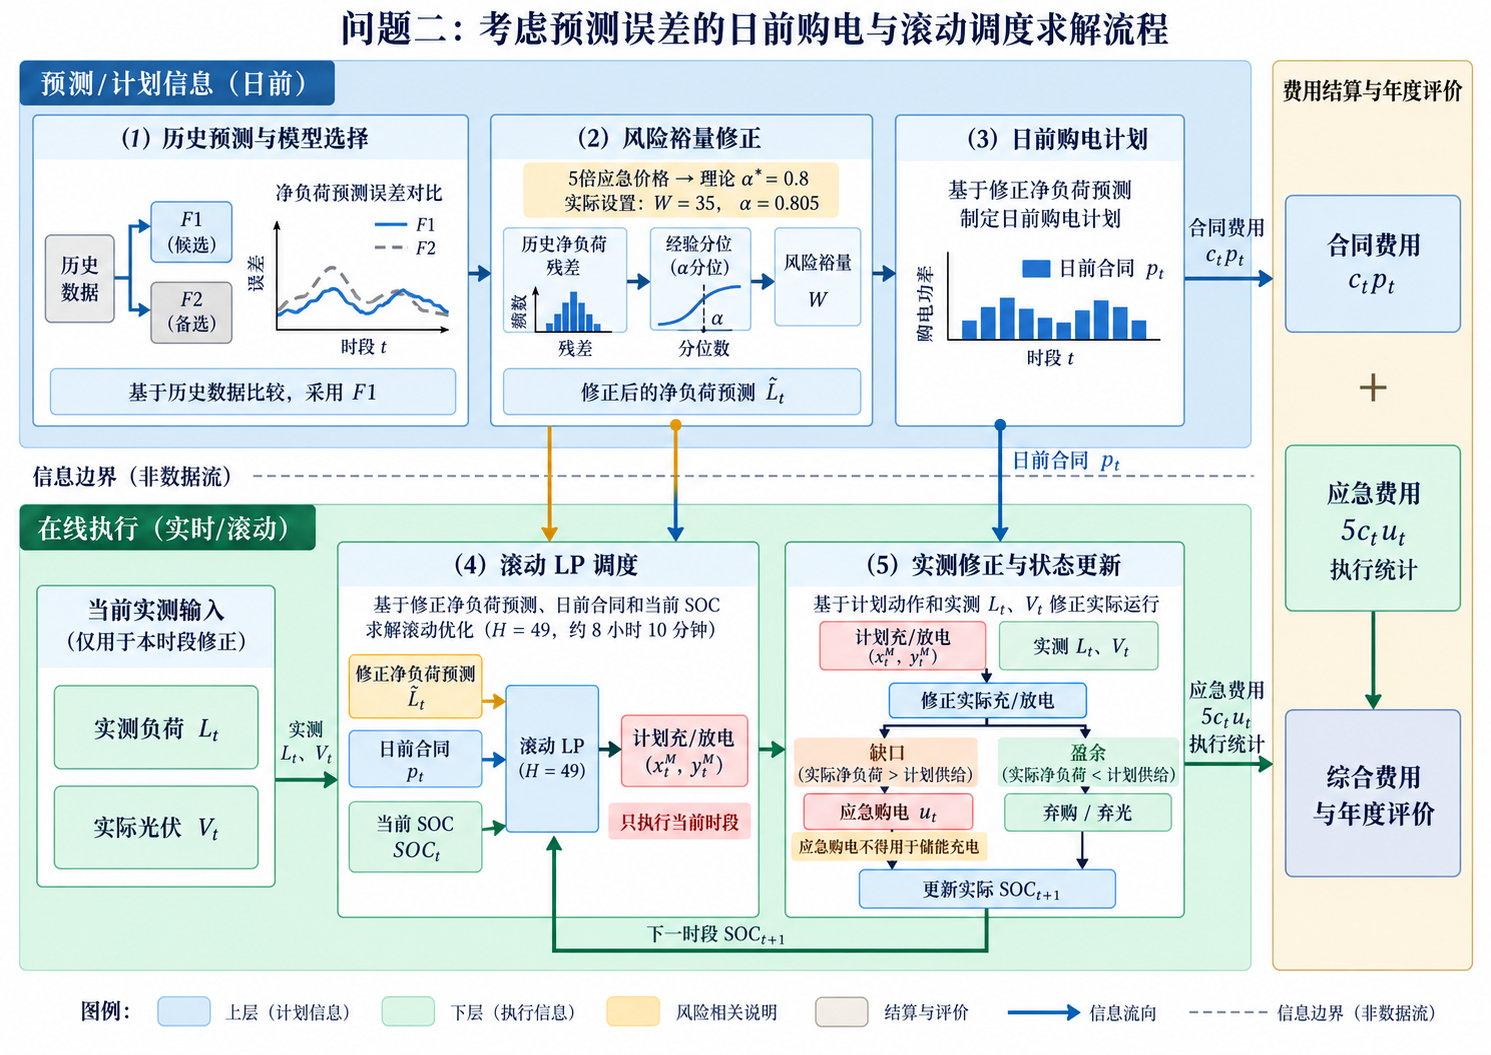
\includegraphics[width=0.78\textwidth]{figures/q2-flow.png}
\caption{问题二求解流程：预测误差修正、日前购电计划与滚动调度}\label{fig:q2-flow}\end{figure}
\subsection{基于历史数据的预测模型}
所有预测只使用目标日之前的数据，光伏功率预测的一般方法与误差来源可参见综述\cite{antonanzas2016review}。记目标日为$d$、同时段为$t$。F1利用负荷的周周期和光伏的近期平均：
\begin{equation}
\widehat L^{F1}_{d,t}=L_{d-7,t},\qquad
\widehat V^{F1}_{d,t}=\frac{1}{7}\sum_{k=1}^{7}V_{d-k,t}.
\label{eq:f1}
\end{equation}
F2以7、14、21日前同时段负荷的中位数抑制单周异常，光伏仍使用近期7日均值：
\begin{equation}
\widehat L^{F2}_{d,t}=\operatorname{median}(L_{d-7,t},L_{d-14,t},L_{d-21,t}).
\label{eq:f2}
\end{equation}
样本不足时，F1和F2均只使用目标日之前已经存在的历史，并按可用历史数据构造。误差指标定义为
\begin{equation}
\mathrm{MAE}=\frac1n\sum_{i=1}^{n}|z_i-\widehat z_i|,\qquad
\mathrm{RMSE}=\sqrt{\frac1n\sum_{i=1}^{n}(z_i-\widehat z_i)^2}.
\label{eq:error-metrics}
\end{equation}
\begin{table}[htbp]\centering\caption{两类基础预测误差对比}\label{tab:forecast-error}
\begin{tabular}{lrrrr}\toprule 模型&负荷MAE&光伏MAE&净负荷MAE&净负荷RMSE\\\midrule
F1&176.80&153.40&273.35&389.97\\F2&187.90&153.40&284.35&403.25\\\bottomrule
\multicolumn{5}{c}{单位：kW。}\end{tabular}\end{table}
\begin{figure}[htbp]\centering
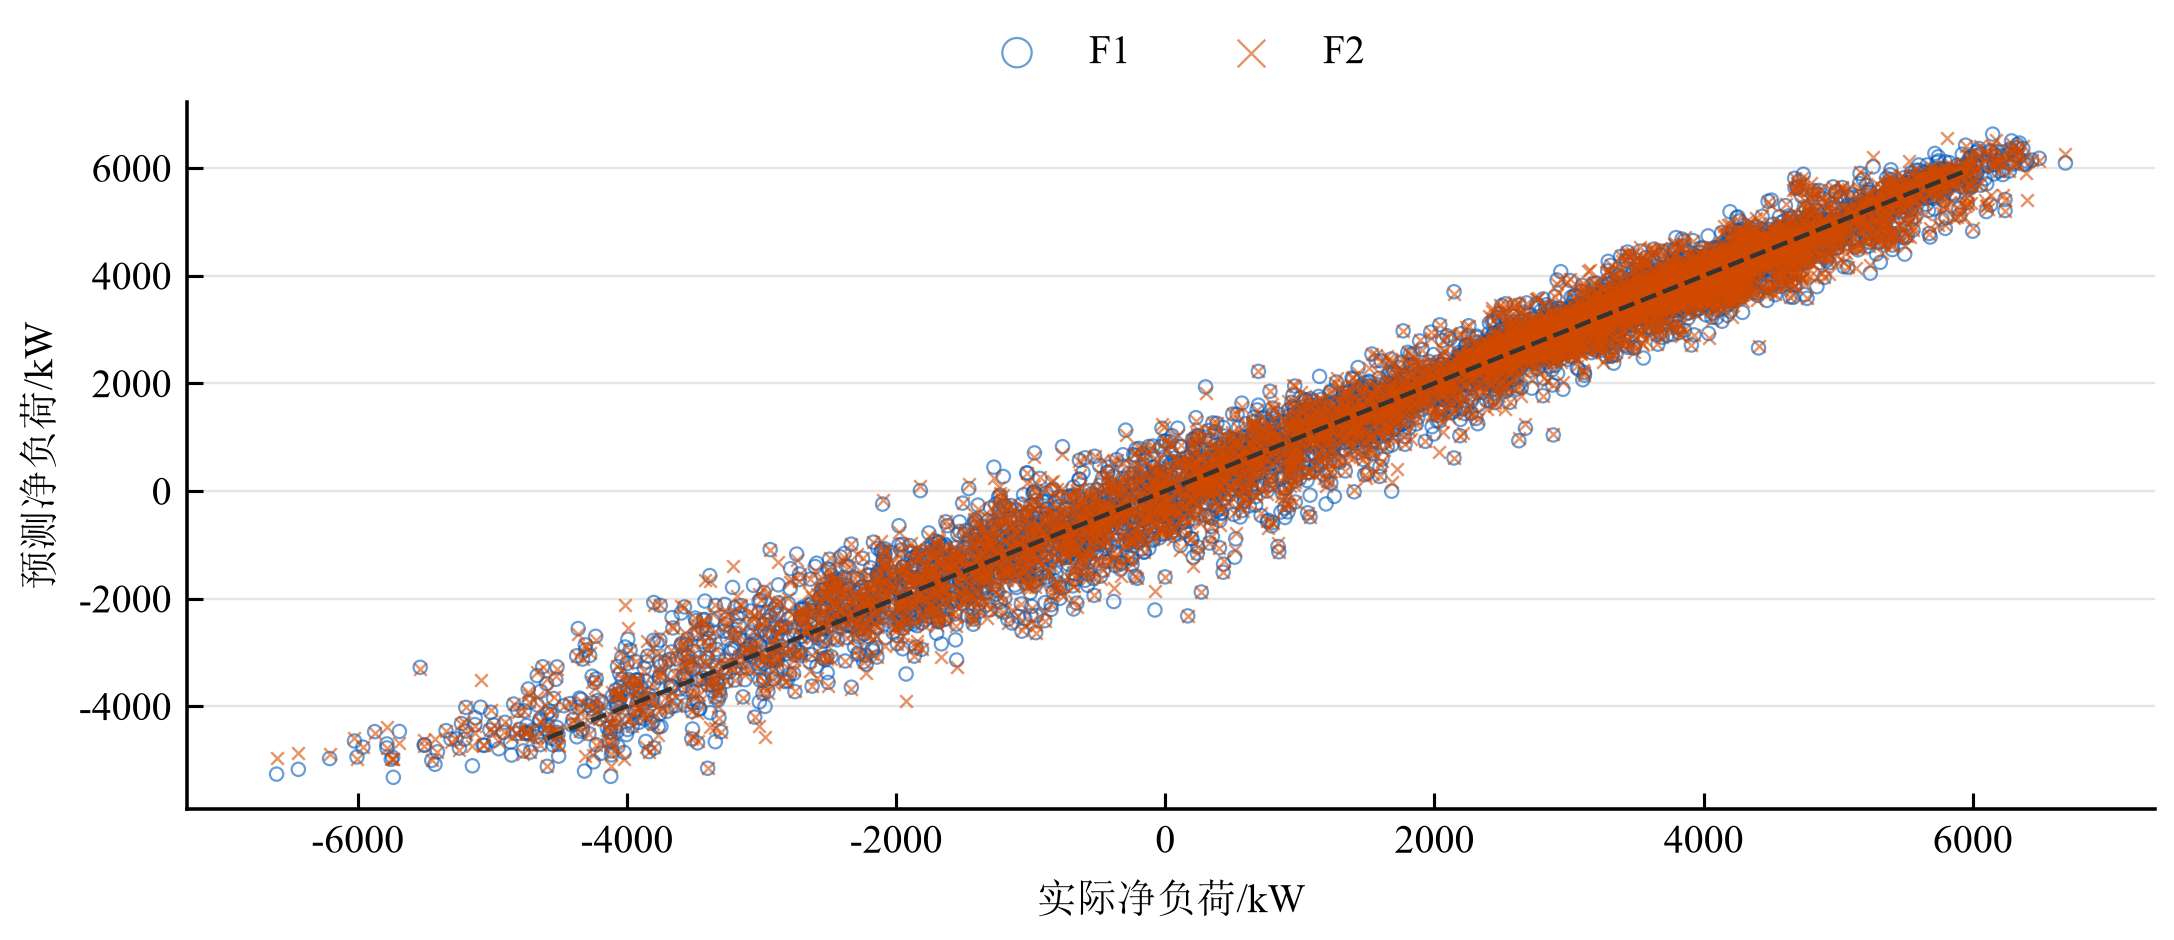
\includegraphics[width=0.96\textwidth]{figures/q2-diagnostics.png}
\caption{基础预测模型的拟合与残差分布诊断}\label{fig:q2-diagnostics}\end{figure}
图\ref{fig:q2-diagnostics}用于比较两种基础预测的拟合表现及残差分布。

由表\ref{tab:forecast-error}可得，F1的净负荷MAE比F2低$11.00\ \mathrm{kW}$。F1用目标日前第7天的同一时段负荷代表目标日负荷，光伏则取前7天同一时段的平均值；F2只把负荷部分改为第7、14、21天同一时段的中位数，光伏预测仍与F1相同。问题二比较F1和F2，是为了单独观察负荷预测构造方法对净负荷风险的影响，最终采用误差较小的F1。

\subsection{基于历史误差分位数的风险裕量修正}
令$\widehat N_{d,t}=\widehat L_{d,t}-\widehat V_{d,t}$，历史残差为
\begin{equation}e^N_{j,t}=N_{j,t}-\widehat N_{j,t},\qquad j<d.\label{eq:q2-residual}\end{equation}
用最近$W$个已完成日构造
\begin{equation}\widetilde N_{d,t}=\widehat N_{d,t}+Q_\alpha\{e^N_{j,t}:d-W\le j<d\}.\label{eq:q2-safe}\end{equation}
按式\eqref{eq:q2-safe}得到修正后的净负荷预测后，通过
\begin{equation}\widetilde V_{d,t}=\max(\widehat V_{d,t},-\widetilde N_{d,t},0),\quad
\widetilde L_{d,t}=\widetilde V_{d,t}+\widetilde N_{d,t}\label{eq:q2-reconstruct}\end{equation}
保持重构后的负荷和光伏非负。

由于加入风险裕量后的净负荷预测可能为负，计算时将其重新表示为非负的负荷预测和光伏预测。该处理只改变分解方式，不改变净负荷本身，因此不影响供需缺口的计算。
\begin{figure}[htbp]\centering

\includegraphics[width=0.96\textwidth]{figures/q2-safe.png}
\caption{基础预测、修正后的净负荷预测与实际净负荷}\label{fig:q2-safe}\end{figure}
图\ref{fig:q2-safe}对比了基础预测、风险修正结果与实际净负荷。

经验分位不要求残差服从正态分布。它把部分历史正偏差加入基础预测：$\alpha$较低时低估净负荷的风险较大，$\alpha$较高时计划购电量和弃购量会增加；$W$控制所使用历史误差的时间范围。分位水平$\alpha$由计划电价与紧急购电价格的比值确定，下面的命题给出这一关系。

\begin{proposition}[5倍应急价格对应的报童分位]\label{prop:q2-newsboy}
考虑单个时段。计划购电价格为$c>0$，计划购电量为$p$，该时段的实际净负荷$N$（负荷减去光伏）为随机变量，剩余供电缺口按$5c$紧急购电。该时段的期望费用为
\begin{equation}J(p)=cp+5c\,\mathbb{E}\big[(N-p)^+\big],\label{eq:newsboy-cost}\end{equation}
其中$(N-p)^+=\max(N-p,0)$为缺口电量。记$N$的分布函数为$F(\cdot)$，则独立决策的最优计划购电量为
\begin{equation}p^\ast=Q_{\alpha^\ast}(N),\qquad
\alpha^\ast=1-\frac{c}{5c}=0.8,\label{eq:newsboy-quantile}\end{equation}
即计划购电量应取净负荷的$0.8$分位。
\end{proposition}
\begin{proof}
式\eqref{eq:newsboy-cost}中只有第二项依赖于$p$。由莱布尼茨法则，
\begin{equation}J'(p)=c-5c\,\mathbb{P}(N>p)=c\big[1-5\big(1-F(p)\big)\big].\label{eq:newsboy-foc}\end{equation}
令$J'(p)=0$得$F(p)=1-1/5=0.8$，即$p=Q_{0.8}(N)$。对式\eqref{eq:newsboy-foc}再求导得$J''(p)=5c\,f(p)\ge0$，故$J$为凸函数，该驻点是全局最小值点；$N$取离散分布时按次梯度理解，结论不变。
\end{proof}

命题\ref{prop:q2-newsboy}与报童模型的分位解一致\cite{khouja1999singleperiod,petruzzi1999pricing}，其边际含义是：多买1度计划电要支付$c$，少买1度计划电则以$1-\alpha$的概率支付$5c$，两种边际代价相等时分位水平为$1-1/5=0.8$。因此计划购电量要在基础预测上加入对应$0.8$分位的风险裕量，以降低低估净负荷导致的高价紧急购电。实际计算中净负荷分布未知，本文用最近$W=35$日的同槽历史残差经验分位数实现这一分位水平；受有限样本影响，实际取值与理论分位略有差别，问题二取$\alpha=0.805$。命题针对单个时段，全年计算中储能带来的跨时段耦合由第\ref{subsec:q2-rolling}节的滚动优化处理。

\subsection{购电计划、滚动调度与年度结果}
每天0:00求解日前合同
\begin{equation}\min\sum_{t=1}^{144}c_tp_t-\lambda(S_{145}-S_{\min}),\label{eq:q2-contract}\end{equation}
式\eqref{eq:q2-contract}的第一项是当天必须支付的合同费用，第二项用于赋予有限时域末SOC以机会价值，鼓励保留可跨越午夜的电量；$\lambda$仅用于边界引导，不计入实际费用。本文取$H=49$，表示每次从当前时段向前考虑49个10分钟时段，即约8小时10分钟。这个长度使当前决策能够在已知分时电价和已发布预测的范围内统筹当天后续一段时间的供需与价格安排，同时仍在下一时段以新的实际SOC重新计算。优化只执行当前时段的调度决策，后续决策随实际状态更新。实际购电费用为
\begin{equation}C_2=\sum_t(c_tp_t+5c_tu_t).\label{eq:q2-cash}\end{equation}
其中$c_tp_t$无论计划购电是否全部使用都要支付，$5c_tu_t$只在实际供电缺口发生时产生；弃购成本已经包含在前一项中，不能再次收费。滚动目标只处理题目给定的能量调度和购电费用，不另行引入随机控制机制。

\subsection{滚动调度与实测修正}\label{subsec:q2-rolling}
在时刻$t$，滚动LP以未来集合$\mathcal H_t=\{t,\ldots,\min(t+H-1,144)\}$为范围，已签合同$g_\tau$视为常量，优化充放电、光伏利用、弃购、应急购电和SOC：
\begin{equation}
\min \sum_{\tau\in\mathcal H_t}5\widehat c_\tau u_\tau
+\varepsilon\sum_{\tau\in\mathcal H_t}(x_\tau+y_\tau)-\lambda S_{\mathrm{end}},
\label{eq:rolling-obj}
\end{equation}
并满足式\eqref{eq:soc}和式\eqref{eq:bus-balance}。合同费用在本阶段已是沉没成本，故滚动目标只需最小化未来应急费用与末态机会成本；$\varepsilon$仅用于在多重最优解中减少不必要的充放电循环。

本文采用滚动LP处理在线决策。滚动LP在每个时刻依据$\mathcal I_{d,t}$形成当前可执行的调度决策。$H$决定当前调度决策考虑的未来范围；较大的$H$有利于在连续时段之间安排储能，也会使较远时段的预测进入当前优化。

采用这种滚动优化有明确的物理原因。若使用单步贪心规则，当前时段通常只比较当下的购电、充电或放电代价，无法把一次充放电对下一时段SOC的影响纳入同一决策。滚动LP则把未来$H$个时段的价格、预测供需和SOC边界同时放入约束与目标：例如当前低价时段的充电会占用功率上限和储能容量，但可能减少后续高价时段的购电；当前放电也会减少后续可用储能。因而，滚动LP能够在不使用未来实测数据的前提下比较当前动作对后续可行性和费用的影响，并在下一时段用新的实际SOC重新修正计划。它适用于本题具有储能跨时段耦合和分时电价的系统，这类滚动时域方法在微网能量管理中已有广泛应用\cite{silvente2015rolling,elkazaz2020ems}。

在问题二中，$H=49$覆盖约8小时10分钟，足以把日内连续时段的储能安排纳入当前计划。需要说明的是，该时域内的未来时段只使用决策时刻已发布的预测；实测负荷与光伏在实际执行后才进入修正环节，因此时域长度只决定对未来预测的利用范围，并不改变各时段的可用信息。

设LP给出的当前时段的调度决策为$(x_t^M,y_t^M)$。获得实测负荷与光伏后，根据实际电力盈余和缺口修正执行量：
\begin{align}
x_t^E&=\min\{x_t^M,(g_t+V_t-L_t)^+\},\label{eq:clip-charge}\\
y_t^E&=\min\{y_t^M,L_t+x_t^E\},\label{eq:clip-discharge}\\
b_t&=L_t+x_t^E-y_t^E-g_t-V_t.\label{eq:clip-gap}
\end{align}
若$b_t\ge0$，则$u_t=b_t,w_t=0,v_t=V_t$；若$b_t<0$，则$u_t=0$，并将$-b_t$依次解释为未利用合同与未利用光伏。该修正保证应急电只补实际供电缺口，不被用于主动充电；时段结束时的实际SOC再由式\eqref{eq:soc}传入下一时段。

334天总费用为$14786101.35$元，合同电量为$22382650.65\ \mathrm{kWh}$。其中计划购电费用为$13665855.74$元，应急费用为$1120245.61$元；应急购电量为$245483.29\ \mathrm{kWh}$，弃购量为$1596110.94\ \mathrm{kWh}$，年末SOC为$10731.91\ \mathrm{kWh}$。应急费用占总费用的$7.58\%$，说明风险修正虽显著减少了极端缺口的经济影响，但预测误差仍是年度成本的重要组成。

合同电量大于最终有效外购供能时，修正后的净负荷预测预留的一部分转化为弃购，供需平衡仍由逐时段方程保证。应急购电量只占合同电量约$1.10\%$，但按5倍电价结算，对总费用贡献达到$7.58\%$。这说明风险裕量需要在低估净负荷造成的高价应急购电和已付费冗余之间取得平衡。

月度结果显示，12月费用最高，为$1788158$元；6月应急购电量最高，为$45846.13\ \mathrm{kWh}$。费用峰值与应急量峰值不完全重合，说明月度成本同时受基础负荷、电价时段分布、合同冗余和应急缺口影响，不能仅用应急电量解释。

\begin{figure}[htbp]\centering

\includegraphics[width=0.96\textwidth]{figures/q2-days.png}
\caption{问题二四个代表日的购电与SOC小倍图}\label{fig:q2-days}\end{figure}
图\ref{fig:q2-days}显示代表日内购电与SOC轨迹的共同结构及差异。

\begin{table}[htbp]\centering\small
\caption{问题二、三四个代表日结果}\label{tab:representative-days}
\begin{tabular}{lrrrr}\toprule
日期&Q2费用/元&Q2应急/kWh&Q3费用/元&Q3应急/kWh\\\midrule
2025-03-20&45158.05&542.74&46105.00&568.04\\
2025-06-21&24282.59&9.36&22415.54&49.31\\
2025-09-23&47616.38&600.29&46491.82&474.10\\
2025-12-21&66632.03&234.75&66196.76&391.83\\\bottomrule
\end{tabular}\end{table}

表\ref{tab:representative-days}中6月21日费用最低、12月21日最高，符合光伏和净负荷的季节差异。Q3未在所有日期优于Q2，且两题预测源和结算规则不同，因此模型价值以在同一问题下比较不同预报方案为准，不由跨题单日差值判断。

为便于核对题目要求的指定日期结果，表\ref{tab:q2-selected}给出问题二六个指定时段的计划购电量，表\ref{tab:q2-blocks}给出四小时聚合的充放电量及日初、日末储电量，表\ref{tab:q2-emergency}给出应急购电发生的时间段和电量。
\begin{table}[htbp]\centering\scriptsize
\caption{问题二四个代表日指定时段计划购电量}\label{tab:q2-selected}
\begin{tabular}{lrrrrrr}\toprule 日期&10:00&12:00&14:00&16:00&18:00&20:00\\\midrule
2025-03-20&0.00&622.11&0.00&505.05&713.88&0.00\\
2025-06-21&0.00&0.00&0.00&258.54&56.78&0.00\\
2025-09-23&0.00&538.75&0.00&583.27&785.94&0.00\\
2025-12-21&0.00&1012.37&0.00&851.75&750.79&0.00\\\bottomrule
\multicolumn{7}{c}{单位：kWh；每列为该时刻起始的10分钟时段。}\end{tabular}\end{table}

\begin{table}[htbp]\centering\scriptsize
\caption{问题二四个代表日四小时充放电及储电量}\label{tab:q2-blocks}
\begin{tabular}{llrrr}\toprule 日期&时间段&充电量/kWh&放电量/kWh&日初--日末储电量/kWh\\\midrule
2025-03-20&0:00--4:00&0.00&0.00&10800.00--10795.24\\
2025-03-20&4:00--8:00&0.00&5499.86&10800.00--10795.24\\
2025-03-20&8:00--12:00&5900.91&3122.72&10800.00--10795.24\\
2025-03-20&12:00--16:00&5283.31&436.64&10800.00--10795.24\\
2025-03-20&16:00--20:00&0.00&5388.59&10800.00--10795.24\\
2025-03-20&20:00--24:00&10252.91&2920.55&10800.00--10795.24\\
2025-06-21&0:00--4:00&0.00&2482.63&10800.00--10800.00\\
2025-06-21&4:00--8:00&0.00&5366.66&10800.00--10800.00\\
2025-06-21&8:00--12:00&6224.02&0.00&10800.00--10800.00\\
2025-06-21&12:00--16:00&3482.98&13.38&10800.00--10800.00\\
2025-06-21&16:00--20:00&0.00&5234.59&10800.00--10800.00\\
2025-06-21&20:00--24:00&9531.47&2485.90&10800.00--10800.00\\
2025-09-23&0:00--4:00&0.00&0.00&10760.83--10793.77\\
2025-09-23&4:00--8:00&43.52&5804.35&10760.83--10793.77\\
2025-09-23&8:00--12:00&5817.31&2823.94&10760.83--10793.77\\
2025-09-23&12:00--16:00&5004.29&178.42&10760.83--10793.77\\
2025-09-23&16:00--20:00&0.00&5602.91&10760.83--10793.77\\
2025-09-23&20:00--24:00&10426.13&2806.64&10760.83--10793.77\\
2025-12-21&0:00--4:00&0.00&0.00&10756.53--10800.00\\
2025-12-21&4:00--8:00&881.63&1508.33&10756.53--10800.00\\
2025-12-21&8:00--12:00&5655.40&7806.67&10756.53--10800.00\\
2025-12-21&12:00--16:00&8333.33&2690.88&10756.53--10800.00\\
2025-12-21&16:00--20:00&0.00&5512.67&10756.53--10800.00\\
2025-12-21&20:00--24:00&10315.06&2842.53&10756.53--10800.00\\\bottomrule
\multicolumn{5}{c}{注：日初、日末储电量在同一日期的六个区间行中重复列示，表示全天边界。}\end{tabular}\end{table}

\begin{table}[htbp]\centering\scriptsize
\caption{问题二四个代表日应急购电时段}\label{tab:q2-emergency}
\begin{tabular}{llr}\toprule 日期&购电时间段&购电量/kWh\\\midrule
2025-03-20&0:20--0:30&1.94\\
2025-03-20&1:00--1:40&116.54\\
2025-03-20&3:10--3:30&36.11\\
2025-06-21&1:20--1:30&1.70\\
2025-06-21&1:50--2:00&1.24\\
2025-06-21&4:00--4:10&0.61\\
2025-09-23&0:40--0:50&13.55\\
2025-09-23&2:10--2:20&14.23\\
2025-09-23&4:50--5:10&38.37\\
2025-12-21&3:00--3:10&7.54\\
2025-12-21&3:30--3:50&65.05\\
2025-12-21&10:30--10:50&28.95\\\bottomrule\end{tabular}\end{table}

\section{问题三：基于日内预报更新的购电调整}
问题三按0:00、6:00、12:00和18:00四个时点获得光伏预报。每个时段的最终购电量只相对0:00的原计划结算一次；中间更新只改变尚未执行时段的购电量。
\subsection{决策时序与信息边界}
一天内共有四个预报版本，新预测只能在规定的发布时间获得。0:00版本用于形成初始计划购电量$p$；6:00、12:00和18:00时，新版本只影响尚未执行的时段，已执行时段不再调整。每次预报更新先读取上一时段结束后的实际SOC，再调整剩余时段的购电量，最后进入下一时段的滚动调度。
\subsection{官方预报校正与分层风险}
对目标日$d$、发布时刻$r$和提前期$h$，使用历史同版本误差校正：
\begin{equation}\widehat V^{\mathrm{cal}}_{d,r,h}=\max\left(0,\widehat V^{\mathrm{raw}}_{d,r,h}+\operatorname{mean}_{j<d}e^V_{j,r,h}\right).\label{eq:q3-calibrate}\end{equation}
校正后插值到10分钟网格。根据提前期将误差分组，分别设置风险裕量；提前期越长，预测误差通常越大，因此相应的风险裕量也随之增大。具体采用六层：$0$--$1$小时、$1$--$2$小时、$2$--$3$小时、$3$--$4$小时、$4$--$5$小时和$5$--$6$小时；提前期超过$6$小时的目标时段统一归入第六层。因此，0:00版本覆盖的6--24小时部分使用第六层风险尺度，后续版本中仍超过6小时的远期时段也按同一层处理。这样既使用了附件3提供的远期预报，又避免为每个小时单独估计样本不足的风险分位。

具体地，令$s_h$为提前期$h$对应残差的经验均方根尺度，标准化残差为$z_{j,r,h}=e^V_{j,r,h}/s_h$，则风险裕量可写为
\begin{equation}
R_{d,r,h}=s_h Q_{\alpha}\{z_{j,r,h}:d-W\le j<d\},\qquad W=35,\ \alpha=0.7725.
\label{eq:q3-stratified}
\end{equation}
式\eqref{eq:q3-stratified}先用$s_h$消除不同提前期的误差量级，再在同层标准化样本上估计共同分位，最后乘回目标提前期尺度。这样既保留“越远期误差通常越大”的结构，又避免每个提前期单独估计分位时样本过少。校正后的1小时、6小时误差MAE分别约为$19.38\ \mathrm{kW}$和$92.71\ \mathrm{kW}$，其增长趋势为不同提前期的误差水平提供了直接数据依据。
\begin{figure}[htbp]\centering

\includegraphics[width=0.96\textwidth]{figures/q3-forecast-quality.png}
\caption{不同发布时间下的光伏预报误差与风险尺度}\label{fig:q3-forecast-quality}\end{figure}
图\ref{fig:q3-forecast-quality}展示预报误差随提前期变化的尺度差异。


\subsection{基于日内预报更新的购电调整}
0:00生成初始计划购电量$p_t$；6:00、12:00和18:00保持已执行时段不变，并以当时的实际SOC重新计算剩余时段的购电量。令
\begin{equation}q_t=p_t+\delta_t^+-\delta_t^-,\qquad\delta_t^+,\delta_t^-\ge0.\label{eq:q3-adjust}\end{equation}
剩余时域目标为
\begin{equation}\min\sum_{t\in\mathcal T_r}[c_tp_t+1.5c_t\delta_t^+-0.5c_t\delta_t^-]-\lambda_r(S_{145}-S_{\min}).\label{eq:q3-update-obj}\end{equation}
最终调整购电量始终相对0:00计划购电量结算一次：
\begin{equation}C_{3,t}=c_t\min(p_t,q_t)+1.5c_t(q_t-p_t)^++0.5c_t(p_t-q_t)^++5c_tu_t.\label{eq:q3-cash}\end{equation}

式\eqref{eq:q3-cash}中的调账费用具有清楚的边际含义。暂不考虑紧急购电项，若$q_t<p_t$，则
\begin{equation}
c_t\min(p_t,q_t)+0.5c_t(p_t-q_t)=0.5c_t p_t+0.5c_t q_t,
\end{equation}
因此减少最终购电量一个单位时，费用相应减少$0.5c_t$；若$q_t>p_t$，则费用为
$c_tp_t+1.5c_t(q_t-p_t)$，增加一个单位最终购电量需增加$1.5c_t$。也就是说，关于$q_t$的边际费用在$q_t<p_t$时为$0.5c_t>0$，在$q_t>p_t$时为$1.5c_t>0$，在$q_t=p_t$处取相应的左右边际值。该分段关系表明，公式结算的是最终购电量相对于原计划的差额：下调部分按$0.5c_t$计费，上调部分按$1.5c_t$计费，并不存在“原计划全额付费后再对下调量重复罚款”的倒挂解释。

每个时段的最终调整购电量只相对0:00的原计划购电量结算一次。中间更新只改变尚未执行时段的最终购电量，不将多次滚动优化的目标值直接相加，因此不会重复计费。

在相邻预报发布时点之间，调度方法以$H=6$即1小时为滚动时域。每次LP同时考虑未来6个时段的价格、修正后的净负荷预测和SOC可行域，只执行当前时段的调度决策。较短时域能够降低尚未更新的远期预测对当前调度决策的影响，也与6小时一次的官方预报更新形成互补。
\begin{figure}[htbp]\centering

\includegraphics[width=0.96\textwidth]{figures/q3-contract.png}
\caption{问题三代表日的事件驱动合同调整与SOC轨迹}\label{fig:q3-contract}\end{figure}
图\ref{fig:q3-contract}给出代表日的合同更新事件与SOC响应。

\subsection{滚动优化相对贪心调度的合理性}
本文采用具有模型预测控制（MPC）基本形式的滚动优化\cite{hu2021mpc,cominesi2018two,schwenzer2021mpc}：每次根据当前储能状态和已发布预测，规划未来若干时段，只执行当前时段的调度决策，随后利用新的实际SOC和预报信息重新计算。SOC递推使当前充放电量影响后续可行域；计划购电、向上调整、向下调整和紧急购电的价格不同，也需要同时比较当前供电与后续费用。

例如，连续两个时段都存在供电缺口且储能只能在其中一个时段放电时，若后一时段的紧急购电单价更高，把储能留到后一时段可少支付$(r_2-r_1)E$。这说明逐时段只处理当前缺口可能忽略储能的后续价值。表\ref{tab:q3-horizon}中$H=1$的样本费用最低，$H=6$仅高$4273.26$元（$0.029\%$）。本文仍取$H=6$作为主方案：它保留了一个小时内连续时段的储能安排，使一次决策能够看到充放电动作对后续SOC和供需缺口的影响，并与6小时一次的官方预报发布时间形成清晰的滚动周期。$H=1$的费用略低是该年度样本下的数值结果，不能说明单步规则在其他样本或其他约束下普遍更优；因此这里把$H=6$作为兼顾费用和多时段可行性安排的正式参数，而不把它表述为费用最优。

合同调整的经济逻辑由三个价格倍率共同决定。向上调整按$1.5c_t$计费，向下调整按$0.5c_t$计费，实际供电缺口按$5c_t$应急购电。更新LP据此比较保留合同、上调、下调和承担应急风险的代价。实际累计上、下调量接近但发生时段不同，说明风险在各时段之间重新分配，整日合同没有单向变化。

\subsection{结果与样本内费用比较}
本文主方案固定参数下的总费用为$14664345.40$元，低于问题二的$14786101.35$元，减少$121755.95$元；应急购电量为$210761.48\ \mathrm{kWh}$，比问题二的$245483.29\ \mathrm{kWh}$减少$34721.81\ \mathrm{kWh}$。在问题三内部，使用全部日内预报相对不使用日内新预报的样本内费用减少$566030.72$元。

0:00计划购电量为$21702724.37\ \mathrm{kWh}$，最终调整购电量为$21702916.77\ \mathrm{kWh}$。累计上调量为$513849.94\ \mathrm{kWh}$，累计下调量为$513657.53\ \mathrm{kWh}$，两者基本相抵但发生时段不同；弃购量为$1228166.90\ \mathrm{kWh}$。

表\ref{tab:q3-selected}--表\ref{tab:q3-emergency}给出与问题二相同格式的四个代表日明细。表\ref{tab:q3-selected}同时列出0:00原计划$p_t$和经过日内更新后的最终合同$q_t$，便于直接观察合同调整；表\ref{tab:q3-blocks}中的储电量为该日0:00和24:00的边界值。
\begin{table}[htbp]\centering\scriptsize
\caption{问题三四个代表日指定时段原计划与最终合同}\label{tab:q3-selected}
\begin{tabular}{llrr}\toprule 日期&时段&原计划$p_t$/kWh&最终合同$q_t$/kWh\\\midrule
2025-03-20&10:00--10:10&0.00&0.00\\
2025-03-20&12:00--12:10&549.71&549.71\\
2025-03-20&14:00--14:10&0.00&0.00\\
2025-03-20&16:00--16:10&652.59&605.82\\
2025-03-20&18:00--18:10&718.21&718.21\\
2025-03-20&20:00--20:10&0.00&0.00\\
2025-06-21&10:00--10:10&0.00&0.00\\
2025-06-21&12:00--12:10&0.00&0.00\\
2025-06-21&14:00--14:10&0.00&0.00\\
2025-06-21&16:00--16:10&203.53&163.73\\
2025-06-21&18:00--18:10&0.00&0.00\\
2025-06-21&20:00--20:10&0.00&0.00\\
2025-09-23&10:00--10:10&0.00&0.00\\
2025-09-23&12:00--12:10&362.95&362.95\\
2025-09-23&14:00--14:10&0.00&0.00\\
2025-09-23&16:00--16:10&609.39&565.35\\
2025-09-23&18:00--18:10&783.44&783.44\\
2025-09-23&20:00--20:10&0.00&0.00\\
2025-12-21&10:00--10:10&0.00&0.00\\
2025-12-21&12:00--12:10&979.30&945.70\\
2025-12-21&14:00--14:10&0.00&0.00\\
2025-12-21&16:00--16:10&853.69&858.30\\
2025-12-21&18:00--18:10&750.11&750.11\\
2025-12-21&20:00--20:10&0.00&0.00\\\bottomrule
\multicolumn{4}{c}{单位：kWh；时段标签表示该10分钟区间。}\end{tabular}\end{table}

\begin{table}[htbp]\centering\scriptsize
\caption{问题三四个代表日四小时充放电及日初日末储电量}\label{tab:q3-blocks}
\begin{tabular}{llrrrr}\toprule 日期&时间段&充电量/kWh&放电量/kWh&0:00储电量/kWh&24:00储电量/kWh\\\midrule
2025-03-20&0:00--4:00&0.00&0.00&10800.00&10800.00\\
2025-03-20&4:00--8:00&0.00&6154.48&10800.00&10800.00\\
2025-03-20&8:00--12:00&3970.58&2485.52&10800.00&10800.00\\
2025-03-20&12:00--16:00&6708.75&328.09&10800.00&10800.00\\
2025-03-20&16:00--20:00&43.56&5094.62&10800.00&10800.00\\
2025-03-20&20:00--24:00&10253.90&2928.49&10800.00&10800.00\\
2025-06-21&0:00--4:00&0.00&2944.22&10800.00&10800.00\\
2025-06-21&4:00--8:00&191.07&5150.11&10800.00&10800.00\\
2025-06-21&8:00--12:00&8517.34&0.00&10800.00&10800.00\\
2025-06-21&12:00--16:00&1293.95&7.58&10800.00&10800.00\\
2025-06-21&16:00--20:00&0.00&5541.12&10800.00&10800.00\\
2025-06-21&20:00--24:00&9909.90&2485.90&10800.00&10800.00\\
2025-09-23&0:00--4:00&0.00&0.00&10800.00&10800.00\\
2025-09-23&4:00--8:00&0.00&6591.76&10800.00&10800.00\\
2025-09-23&8:00--12:00&5624.09&2048.24&10800.00&10800.00\\
2025-09-23&12:00--16:00&5445.49&388.79&10800.00&10800.00\\
2025-09-23&16:00--20:00&0.00&5602.91&10800.00&10800.00\\
2025-09-23&20:00--24:00&10391.99&2752.18&10800.00&10800.00\\
2025-12-21&0:00--4:00&0.00&0.00&10800.00&10800.00\\
2025-12-21&4:00--8:00&833.33&1508.33&10800.00&10800.00\\
2025-12-21&8:00--12:00&5218.33&7703.98&10800.00&10800.00\\
2025-12-21&12:00--16:00&7534.09&1792.14&10800.00&10800.00\\
2025-12-21&16:00--20:00&0.00&5434.51&10800.00&10800.00\\
2025-12-21&20:00--24:00&10218.56&2842.53&10800.00&10800.00\\\bottomrule
\end{tabular}\end{table}

\begin{table}[htbp]\centering\scriptsize
\caption{问题三四个代表日应急购电时段}\label{tab:q3-emergency}
\begin{tabular}{llr}\toprule 日期&购电时间段&购电量/kWh\\\midrule
2025-03-20&0:20--0:30&7.34\\
2025-03-20&1:00--1:40&99.45\\
2025-03-20&3:10--3:30&36.04\\
2025-06-21&0:20--0:30&5.36\\
2025-06-21&1:20--1:30&11.72\\
2025-06-21&1:50--2:00&12.69\\
2025-09-23&0:40--0:50&14.46\\
2025-09-23&2:10--2:20&14.35\\
2025-09-23&4:50--5:10&21.85\\
2025-12-21&1:30--1:40&7.73\\
2025-12-21&3:00--3:10&27.03\\
2025-12-21&3:30--3:50&104.82\\\bottomrule\end{tabular}\end{table}

1002次购电量更新均成功，全年所有滚动优化问题均成功求解。修正后的净负荷预测逐时段覆盖率为$76.95\%$，与$\alpha=0.7725$接近；覆盖率提高通常伴随更多弃购，因此参数选择还需结合费用。按提前时间分组设置风险裕量时，总费用比各时段采用同一风险裕量高$8860.56$元，但前者保留了提前期越长、预测误差通常越大的特征。本文同时报告两种方案的结果。

\begin{table}[htbp]\centering\small
\caption{不同日内预报组合的结果比较}\label{tab:q3-ablation}
\begin{tabular}{lrrr}\toprule
预报组合$\mathcal S$&年度费用/元&应急购电/kWh&样本内费用差异/元\\\midrule
$\varnothing$&15230376.12&334601.06&0.00\\
$\{6\}$&15038617.00&266410.12&191759.11\\
$\{12\}$&14746909.96&224631.56&483466.16\\
$\{18\}$&14805047.54&228882.13&425328.58\\
$\{6,12\}$&14679898.82&217968.28&550477.30\\
$\{6,18\}$&14864586.68&218423.74&365789.44\\
$\{12,18\}$&14710994.09&212056.29&519382.03\\
$\{6,12,18\}$&14664345.40&210761.48&566030.72\\\bottomrule
\end{tabular}
\end{table}

表\ref{tab:q3-ablation}的不使用日内新预报的方案保留相同滚动调度方法但屏蔽新版预报。使用全部三个日内预报的方案样本内费用减少$56.60$万元（$3.72\%$）；6:00、12:00和18:00更新的平均边际费用差异分别为$6.15$、$28.41$和$16.27$万元，表明不同更新时间的样本内影响存在差异。
\begin{figure}[htbp]\centering

\includegraphics[width=0.96\textwidth]{figures/q3-ablation.png}
\caption{不同日内预报组合的信息消融结果}\label{fig:q3-ablation}\end{figure}
图\ref{fig:q3-ablation}将不同预报组合的费用与应急购电结果并列比较。
\begin{figure}[htbp]\centering
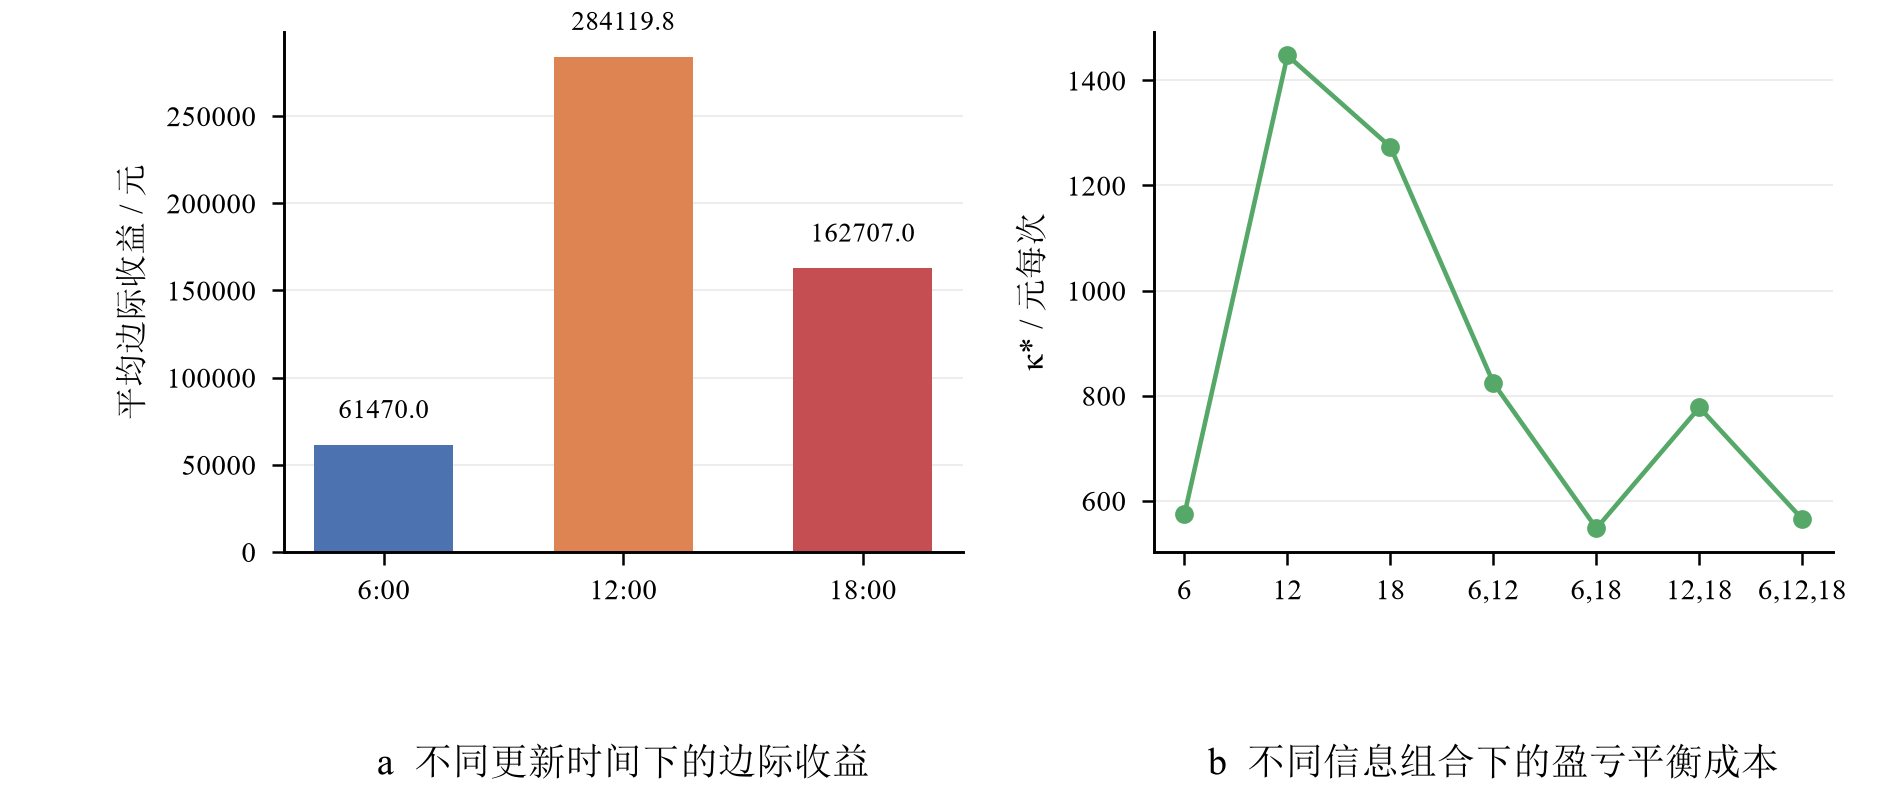
\includegraphics[width=0.96\textwidth]{figures/q3-time-value.png}
\caption{官方更新时间的样本内费用差异与信息组合盈亏平衡成本}\label{fig:q3-time-value}\end{figure}
图\ref{fig:q3-time-value}进一步量化各更新时间的信息价值与盈亏平衡成本。

\subsection{是否需要增加其他预报时点}
题目现有的官方预报只在0:00、6:00、12:00和18:00发布，因此本文首先比较这三个日内更新时点的不同组合。表\ref{tab:q3-ablation}显示，只采用6:00、12:00或18:00中的任一时点，费用均低于不使用日内新预报的方案；同时采用三个时点时，在本年度样本比较中费用最低，为$14664345.40$元，应急购电量也最低，为$210761.48\ \mathrm{kWh}$。这说明在题目已经提供的预报范围内，三个日内时点均具有实际作用，不能仅保留其中一个时点。

对于6:00、12:00和18:00以外的发布时间，现有数据没有提供相应的独立预报版本。为补充考察“其他时刻”，本文选取3:00、9:00、15:00和21:00四个区间中点，每次只向基准事件集合$\mathcal R_0=\{0,6,12,18\}$加入一个候选时点。候选时点采用此前最近一次官方版本的已校正预报曲线作为代理，并完全复用$W=35,\alpha=0.7725,H=6$的合同调整、滚动执行和现金结算流程。该设置仅作为代理敏感性测试，用于衡量代理信息条件下增加一次更新机会的样本内费用差异，不能解释为附件3对新增时点的实测验证，也不能视为真实新增预报信息。

新增预报更新时点的盈亏平衡成本为
\begin{equation}\kappa^*=\frac{C_{\mathrm{old}}-C_{\mathrm{new}}}{\Delta n},\qquad\Delta n>0.\label{eq:kappa}\end{equation}
对使用全部三个日内预报的方案相对不使用日内新预报的方案而言，$\Delta n=1002$，故平均盈亏平衡成本为$564.90$元/次。若实际获得、传输和执行一次更新的综合成本低于该值，全年采用全部日内预报在样本内具有正净收益；若只能选择一个时点，则12:00优先级最高。

对候选时点$r$，每个验证日仅增加一次更新，故以日均费用计算
$\kappa_r^*=C(\mathcal R_0)-C(\mathcal R_0\cup\{r\})$。334天闭环代理回放结果见表\ref{tab:q3-extra-time}。
\begin{table}[htbp]\centering\small
\caption{其他预报时点的单次边际代理测试}\label{tab:q3-extra-time}
\begin{tabular}{crrrrc}\toprule
候选时点&年度费用/元&样本内费用差异/元&$\kappa_r^*$/元每次&正收益天数&结论\\\midrule
3:00&15540003.28&$-875657.88$&$-2621.73$&39/334&不引入\\
9:00&14958681.94&$-294336.54$&$-881.25$&71/334&不引入\\
15:00&14653971.85&10373.54&31.06&171/334&可引入\\
21:00&14613131.18&51214.22&153.34&302/334&不建议（夜间）\\\bottomrule
\end{tabular}
\end{table}
在代理情景下，3:00和9:00虽降低了应急购电量，但合同重算带来的现金费用上升，因而不满足引入判据；15:00的正收益天数为171天，仅略超过半数，可作为谨慎候选。21:00虽然在302天产生正收益，年度样本内费用差异为$51214.22$元，但附件2全年21:00后的6570个时段中实际光伏功率均为$0\ \mathrm{kW}$，此时已经没有可供修正的日照信息。故该收益实质上来自多增加一次基于当前SOC的合同重优化机会，而非21:00光伏预报本身的新增预报信息。实际系统中专门设置21:00光伏预报更新缺乏物理意义，增加通信、计算和交易环节后反而欠妥，因此不予推荐。若取得其他日照时段的独立预报，应替换代理版本后重新回放。

\begin{table}[htbp]\centering\caption{问题三滚动时域折中}\label{tab:q3-horizon}
\begin{tabular}{crr}\toprule
$H$/时段&考虑的未来时长&年度费用/元\\\midrule
1&10分钟&14660072.14\\3&30分钟&14662818.12\\
6&1小时&14664345.40\\12&2小时&14671133.74\\\bottomrule
\end{tabular}\end{table}
由表\ref{tab:q3-horizon}可得，$H=1$的样本费用最低，但$H=6$仅高$4273.26$元（$0.029\%$）。结合上一节关于SOC跨时段耦合、购电责任和预报更新的分析，本文将$H=6$作为样本费用、多时段规划能力和求解速度之间的折中。

\section{问题四：波动电价下的购电策略}
\subsection{基于历史信息的电价预测}
附件4给出实际结算电价，而在0:00制定计划时，该日后续时段的实际电价尚未观测。问题四采用近30日中位数作为0:00的价格基线，即对每个目标时段取最近30天同一时段价格的中位数。四种基准方法误差见表\ref{tab:price-error}；本文保留该比较，但两种合同模式均使用同一近30日中位数基线。该基线是为了保证Q4-2与Q4-3的统一比较口径，并不是分别为两种模式挑选的样本内最优价格预测器。
\begin{table}[htbp]\centering\small\caption{四种0:00基准价格预测方法误差}\label{tab:price-error}
\begin{tabular}{lrrrr}\toprule 基准方法&MAE&RMSE&尖峰MAE&最大绝对误差\\\midrule
昨日同时段&0.08433&0.12384&0.09226&0.53200\\近7日均值&0.08267&0.10527&0.09686&0.49669\\
近30日均值&0.08748&0.11351&0.10835&0.54015\\近30日中位数&0.08328&0.12074&0.09880&0.62360\\\bottomrule
\multicolumn{5}{c}{单位：元/kWh。}\end{tabular}\end{table}
日内只使用已经完成时段的价格误差做修正，修正量按目标时段与当前时刻的距离指数衰减。规划阶段使用预测价格，实际费用按实际电价结算。
\begin{figure}[htbp]\centering

\includegraphics[width=0.96\textwidth]{figures/q4-price-diagnostics.png}
\caption{波动电价预测的拟合与误差分布}\label{fig:q4-price-diagnostics}\end{figure}
图\ref{fig:q4-price-diagnostics}给出各价格基线的拟合与误差分布。

设0:00的近30日中位数价格基线为$\widehat c^{(0)}_{d,t}$，日内时刻$k$之前已完成时段的价格误差为$e^c_{d,j}=c_{d,j}-\widehat c^{(0)}_{d,j}$。本文以这些已完成时段误差的加权平均形成日内修正，并随目标时段距离当前时刻的远近衰减：
\begin{equation}
\widehat c_{d,t\mid k}=\max\left\{10^{-4},
\widehat c^{(0)}_{d,t}+\bar e^c_{d,k}\exp[-(t-k)/18]\right\},\quad t\ge k.
\label{eq:q4-price-correction}
\end{equation}
该式只使用时刻$k$之前已经观察到的价格，附件4中未来时段的实际电价不提前用于决策。下限$10^{-4}$用于避免数值上出现非正价格；实际电价始终只进入最终结算。

四种基准方法的预测误差排序与最终费用排序不完全一致，原因在于MAE对各时段等权，而费用还受高负荷、紧急购电和储能状态影响。为使固定合同与可调合同只比较合同调整方式，二者均采用近30日中位数价格基线。问题二比较F1和F2，是为了考察历史负荷预测方法对净负荷风险修正的影响；问题四的新增因素是波动电价及其预测，因此沿用F1负荷预测并叠加官方光伏预报。若在问题四改用F2，费用差异将同时包含负荷预测方法变化，难以单独比较价格和合同机制，故不继续使用F2。

Q4-2与Q4-3的区别在于购电计划是否允许日内调整。Q4-2在0:00形成合同，之后保持合同不变；Q4-3在0:00形成初始合同，并在6:00、12:00和18:00依据新信息调整尚未执行的时段。两种模式都在滚动LP中使用预测价格和预测的负荷、光伏安排调度，合同调整仍按式\eqref{eq:q3-cash}相对0:00原计划结算一次，最终费用则使用附件4的实际电价。下面的结果表因此同时比较合同调整本身及其对应的实际费用变化。

\subsection{结果比较}
\begin{table}[htbp]\centering\caption{问题四两种模式的年度结果}\label{tab:q4-result}
\begin{tabular}{lrrr}\toprule 模式&总费用/元&应急购电量/kWh&更新次数\\\midrule
Q4-2固定合同&17378687.69&570732.66&0\\Q4-3可调合同&15465962.60&210394.02&1002\\\bottomrule\end{tabular}\end{table}
表\ref{tab:q4-result}显示，Q4-3相对Q4-2的样本内费用减少$1912725.09$元，降幅为$11.01\%$。应急购电减少$360338.64\ \mathrm{kWh}$，降幅为$63.14\%$。这说明波动电价下日内合同调整的样本内费用下降同时来自缺口减少和时段安排优化。

\begin{table}[htbp]\centering\small
\caption{问题四价格基准方法与事后理想信息基准结果}\label{tab:q4-baselines}
\begin{tabular}{lrr}\toprule
价格基准方法&Q4-2费用/元&Q4-3费用/元\\\midrule
昨日同时段&17402307.33&15485837.98\\
近7日均值&17390589.20&15454638.40\\
近30日均值&17400942.40&15455190.24\\
近30日中位数&17378687.69&15465962.60\\
0:00已知实际电价&17300085.39&15383049.81\\\bottomrule
\end{tabular}\end{table}

由表\ref{tab:q4-baselines}可见，四种基于历史信息的基准方法下Q4-2费用极差仅$23619.64$元，Q4-3极差为$31199.58$元，说明合同调整机制的样本内费用优势并不依赖某一个价格预测器。以本文主方案固定参数下的费用与“事后理想信息基准”（假设0:00已知全天实际电价的理想情形）之差定义样本内费用差异，Q4-2与Q4-3分别为$78602.31$元和$82912.80$元，只占各自总费用的$0.45\%$和$0.54\%$。因此波动价格相对固定价格造成的费用变化不能全部归因于预测误差，其中还包含实际电价水平、尖峰位置和光伏缺口的共同作用。

Q4-3在四种基准方法下均比Q4-2低约190万元，说明合同更新机制的样本内费用优势大于在这些简单价格预测器之间切换的优势。

\section{模型检验与灵敏度分析}
\subsection{数值与物理检验}
Q1--Q4逐项检查供需平衡方程、SOC递推、变量边界、充放电状态和跨日连续性。各方案的约束均满足，SOC始终位于$[1200,10800]\ \mathrm{kWh}$，且没有同时充电和放电的时段。问题一中供需平衡残差的最大值为$2.27\times10^{-13}\ \mathrm{kWh}$，该数值仅用于说明计算校验精度；问题二至问题四不再重复列出同类浮点误差。

\subsection{规划--执行偏差与费用核对}
滚动控制中的计划调度决策不要求与实际执行完全相同，因为作出当前时段决策后才读取本时段实测负荷和光伏。本文以计划下一时段SOC与实际SOC的差作为诊断量。Q2、Q3、Q4-2和Q4-3的一步SOC误差MAE分别为$5.33$、$5.06$、$4.80$和$5.16\ \mathrm{kWh}$，相对于$12000\ \mathrm{kWh}$额定容量均不足$0.045\%$；对应最大绝对误差均不超过$284.59\ \mathrm{kWh}$。这说明预测误差会触发必要的时段内修正，但未导致状态轨迹失控。

费用核对时，将计划、调整和紧急购电费用分别汇总，分项之和与逐时段费用之和一致。全文均采用式\eqref{eq:q3-cash}所给的主结算口径：每个时段的最终购电量只相对0:00原计划结算一次，已发生费用不再重复调整。

\subsection{尾部风险与跨月稳定性}
年度平均费用只能反映334天的总体水平，少数极端高费用日可能被平均值掩盖。为评价这种风险，本文在2025年2月1日至12月31日、共334天的逐日费用序列上计算VaR和CVaR（条件风险价值的定义与优化见\cite{rockafellar2000cvar}，其在储能调度中的应用见\cite{khodabakhsh2016cvar}），结果见表\ref{tab:tail-risk}。VaR$_{0.95}$是逐日费用的95\%分位阈值，可理解为费用进入最差约5\%日期时的起始水平；CVaR$_{0.95}$是超过该阈值的高费用日平均值。二者评价的对象都是每天的总费用，分别反映尾部开始位置和尾部平均损失。
\begin{table}[htbp]\centering\small
\caption{主方案日费用尾部风险}\label{tab:tail-risk}
\begin{tabular}{lrrrr}\toprule
方案&日均费用/元&VaR$_{0.95}$/元&CVaR$_{0.95}$/元&最坏日费用/元\\\midrule
Q2&44269.76&66075.35&70048.64&88726.19\\
Q3&43905.23&65177.30&70474.34&77111.50\\
Q4-2&52032.00&87294.40&101705.29&134220.63\\
Q4-3&46305.28&76237.79&83469.29&92033.53\\\bottomrule
\end{tabular}\end{table}
Q3的日均费用为$43905.23$元，低于Q2的$44269.76$元；其最坏日费用也由$88726.19$元降至$77111.50$元，说明在样本内，日内预报更新不仅影响平均水平，也改善了高费用日期的表现。问题四中，Q4-3相对Q4-2的年度总费用减少$1912725.09$元，CVaR减少$18235.99$元，最坏日费用由$134220.63$元降至$92033.53$元。该结果与问题三的结论相互补充：问题三说明日内光伏信息能够降低费用和应急购电量，问题四进一步表明在实际波动电价下，允许调整购电计划还能够降低高费用日的损失。

跨月比较的对象是问题三使用全部三个日内预报与不使用日内新预报的两种方案，比较范围为2025年2月至12月。已有月度结果显示，11个月的日均费用差均为负；7月平均每天费用下降$2889.94$元，12月费用仍下降$473.89$元。因此，信息更新带来的费用下降并不只由某一个月份贡献，且在年度末仍保持正向差异。
\begin{figure}[htbp]\centering
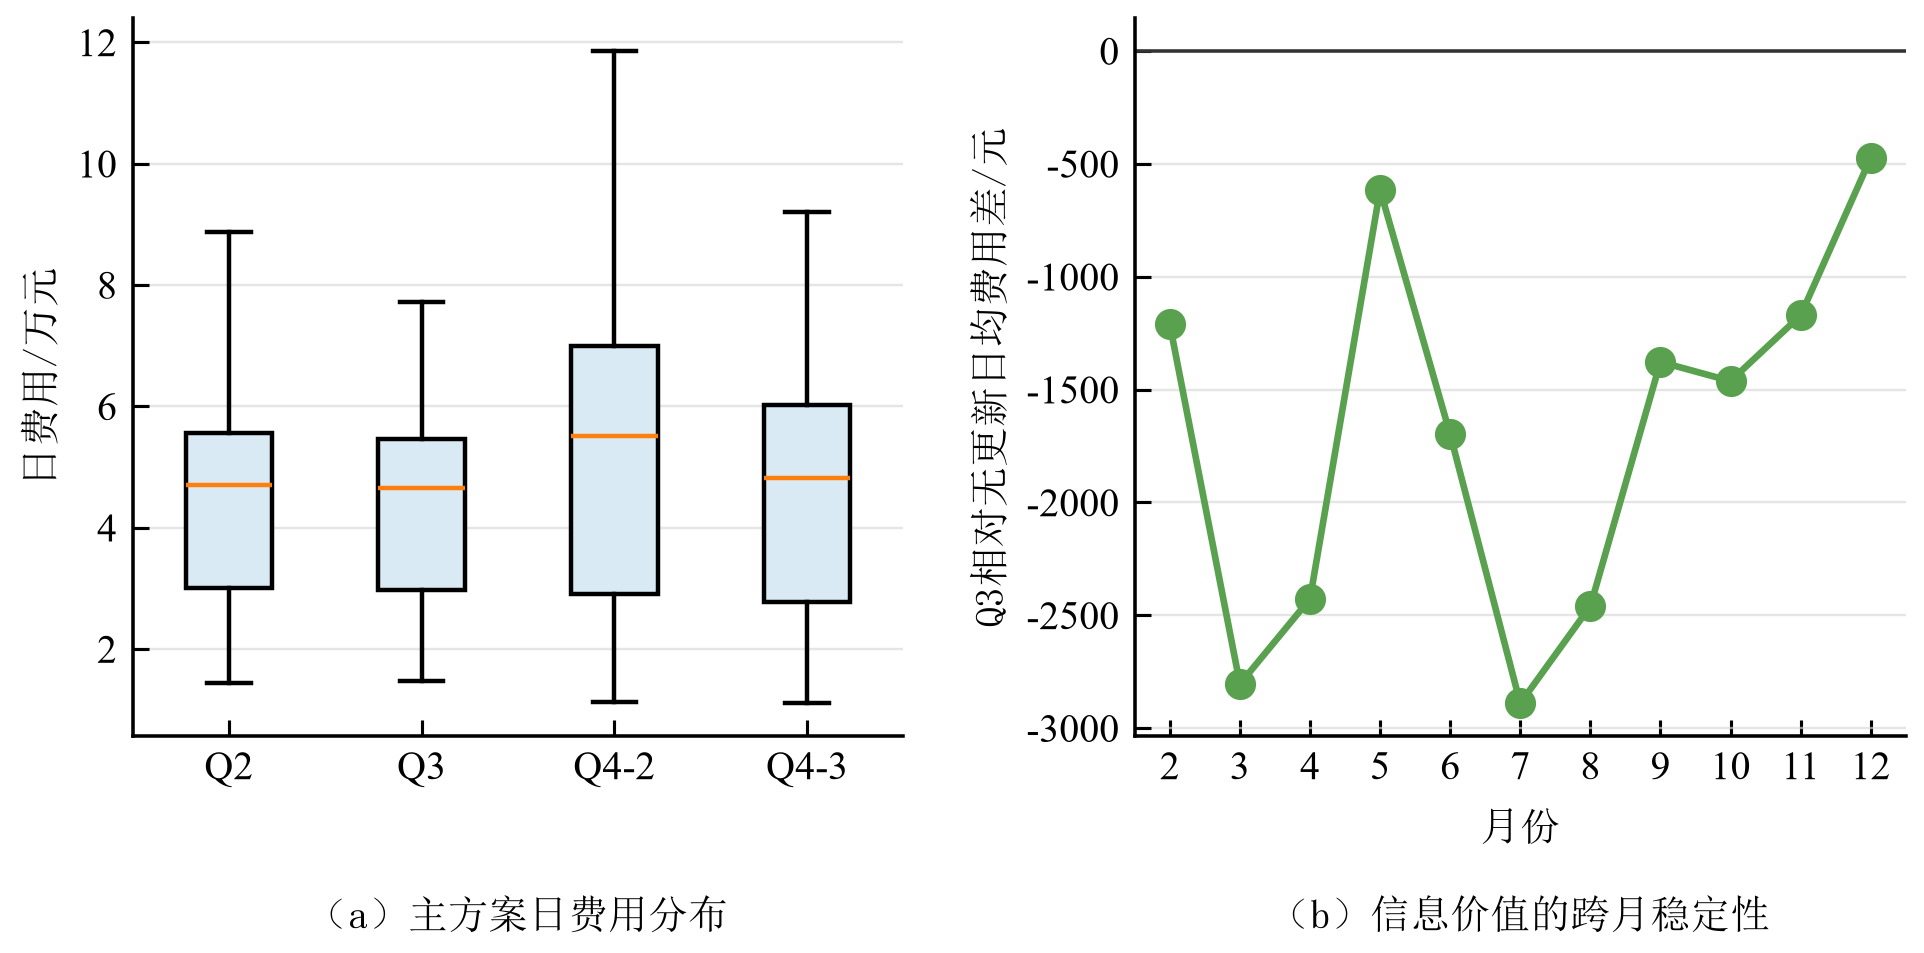
\includegraphics[width=0.96\textwidth]{figures/risk-stability.png}
\caption{主方案日费用尾部风险与跨月稳定性}\label{fig:risk-stability}\end{figure}
图\ref{fig:risk-stability}用于核对尾部风险下降是否由个别月份驱动。

\subsection{结构敏感性}
本节的目的，是判断储能物理参数变化是否会明显改变年度费用、应急购电量及前述结论方向。各情景均保持相同的信息集和主结算口径，只改变一个参数或一组明确给出的参数。
\begin{table}[htbp]\centering\small
\caption{问题二结构敏感性结果}\label{tab:structure-sensitivity}
\begin{tabular}{lrrr}\toprule
情景&年度费用/元&相对基准变化&应急购电/kWh\\\midrule
基准&14786101.35&0.00\%&245483.29\\
$\eta_c=\eta_d=\sqrt{0.9}$&14322473.62&$-3.14\%$&251361.82\\
容量$-20\%$&15392912.44&$+4.10\%$&251029.71\\
容量$+20\%$&14267282.70&$-3.51\%$&250574.68\\
功率$-20\%$&16318749.90&$+10.37\%$&563286.32\\
功率$+20\%$&14738026.27&$-0.33\%$&247951.11\\\bottomrule
\end{tabular}\end{table}

表\ref{tab:structure-sensitivity}先给出效率、容量和充放电功率上限的变化结果；补充结果还比较了初始SOC、预测误差倍率和终端价值倍率。效率改取$\sqrt{0.9}$后，费用下降$3.14\%$，说明效率口径会直接影响储能损耗和总费用。容量减少或增加20\%时，费用分别变化$+4.10\%$和$-3.51\%$，影响小于功率上限变化。功率上限减少20\%使费用上升$10.37\%$、应急购电量增至$563286.32\ \mathrm{kWh}$；增加20\%时费用仅下降$0.33\%$，表明功率上限是表中最敏感的物理参数，功率不足会直接限制储能在关键时段的充放电能力。

初始SOC取额定容量的20\%、50\%或80\%时，正式统计窗口的费用相同，说明1月的连续运行和预热已消除初始状态差异。预测误差倍率$\gamma=0.5,1.5,2$时，费用相对基准分别变化$+12.49\%$、$+1.20\%$和$+4.51\%$；这些结果说明风险裕量大小会改变合同冗余与应急购电之间的平衡。终端价值倍率取0时费用为$21869985.06$元，取1与1.5时结果相同，因此正文采用倍率1作为滚动优化中的末态引导。
\begin{figure}[htbp]\centering

\includegraphics[width=0.96\textwidth]{figures/sensitivity-overview.png}
\caption{物理参数与预测误差的综合敏感性}\label{fig:sensitivity-overview}\end{figure}
图\ref{fig:sensitivity-overview}汇总了关键物理参数与预测误差扰动的影响。
\section{模型评价与推广}
\subsection{模型特点}
本文针对赛题的信息时序、风险费用和结算规则作了以下处理：
\begin{enumerate}
\item 四问采用相同的物理约束和决策时可用信息集$\mathcal I_{d,t}$，仅按题意改变购电量调整权限和电价过程；实测数据在当前时段决策形成后才用于修正和结算。
\item 5倍紧急购电价格使风险裕量具有经济必要性；计划购电量与应急购电量的最优权衡由命题\ref{prop:q2-newsboy}给出，理论分位为$0.8$，实际由历史净负荷误差分位数实现，并以最终参数进行全年逐日模拟。循环能量恒等式用于独立检查计算结果。
\item 0:00计划购电量、最终调整购电量、弃购量和紧急购电量分别记录；每个时段的最终购电量只相对0:00原计划结算一次。
\item 八种预报组合的样本内费用比较、样本内费用差异和$\kappa^*$用于描述各预报时点的样本内影响；事后理想电价信息基准用于报告电价未知情形的样本内费用差异。
\item 问题三和问题四均采用相同的滚动调度方法比较不同预报和合同方案；预报组合对比用于衡量不同预报时点的费用和应急购电量变化。
\end{enumerate}
\subsection{局限与推广}
题面未给并网容量和售电机制，本文假定外购电无上限且不可反送；若实际存在容量限制，应增加$g_t+u_t\le G_{\max}$。经验分位描述历史残差的边际尾部，没有刻画连续多时段预测误差之间的相关性，因此逐时段覆盖率不能解释为整日可靠概率。10分钟聚合忽略时段内测量延迟和功率爬坡，实际应用时需缩短步长或加入延迟状态。上述结论基于2025年历史数据，换用其他年份时需重新检验参数和费用表现。此外，滚动线性规划设置了求解时间上限，极少数时刻可能退回兜底规则；正式模拟中该分支未触发，全部执行决策均来自仅使用已发布预测的线性规划。

按提前时间分组设置风险裕量时，当前样本费用比各时段采用同一风险裕量高$8860.56$元。本文仍采用分组方案，是因为它保留了提前期越长、预测误差通常越大的已有数据特征。问题三中$H=1$的费用略低于$H=6$，说明滚动时域需要在样本费用和多时段规划能力之间折中。

模型可扩展到含风电、可控负荷和多储能的园区微网。新增能源可在供需平衡方程中加入供给变量；新增需求响应则加入移峰变量与舒适度约束。若允许售电或出现负电价，应采用显式充放电互斥的混合整数模型，防止循环套利。微网分层控制的一般背景可参见相关综述\cite{bouzid2015microgrid}。

若获得多年数据，可把当前35日滑动分位替换为季节条件分位或场景树\cite{farzin2017stochastic}，或改用对不确定集合直接优化的鲁棒模型\cite{zugno2015robust,zhang2013robust,alonso2022uncertainty}，并用独立年份选择$W,\alpha,H$；若预报供应商按次收费，可将$\kappa$加入预报获取方案优化，把盈亏平衡分析扩展为0--1选择模型；若园区包含多块电池，可为每块储能分别建立SOC方程，并增加共享并网容量和寿命折损成本。上述扩展仍可沿用本文的购电计划、实际调度和费用结算过程。

\section{结论}
购电计划、实际调度和费用结算三个环节，以及决策时可用信息集$\mathcal I_{d,t}$，构成统一处理四个问题的基础。它们明确了各时刻可使用的信息、购电量调整的生效范围和实际费用的计算口径。

问题一的全天计划购电量为$59482.70\ \mathrm{kWh}$、费用为$35126.95$元，SOC满足边界并回到日初状态。问题二采用F1，风险裕量的分位水平由计划电价与5倍应急价格的比值确定，理论值为$0.8$，实际固定采用$W=35,\alpha=0.805,H=49$，334天总费用为$14786101.35$元；该组参数由同一年度样本回放比较确定，属于样本内参数，其年度指标仅解释为样本内闭环回放结果，应急购电量为$245483.29\ \mathrm{kWh}$。

问题三采用F1与官方光伏预报，主方案固定参数$W=35,\alpha=0.7725,H=6$。相对于问题二的总费用$14786101.35$元，问题三总费用为$14664345.40$元，减少$121755.95$元；应急购电量由$245483.29$降至$210761.48\ \mathrm{kWh}$。在问题三内部，采用全部三个日内预报相对于不使用日内新预报的样本内费用减少$566030.72$元，三次更新的平均盈亏平衡成本为$564.90$元/次。
在其他时刻的单次边际代理测试中，15:00满足正收益及多数日改善判据，但正收益天数仅为171天，故只作为谨慎候选。21:00虽表现出$51214.22$元的样本内费用差异，但全年该时刻之后光伏出力均为零，该差异来自额外合同重优化而非光伏信息，实际中不建议设置该预报时点。

问题四中，固定合同和可调合同费用分别为$17378687.69$元和$15465962.60$元，日内调整使样本内费用减少$1912725.09$元并使应急量降低$63.14\%$。相对事后理想价格信息基准，两种模式的样本内费用差异约为$7.86$万元和$8.29$万元。

尾部风险检验中，Q4-3相对Q4-2的CVaR下降$18235.99$元，说明合同调整同时压缩极端高费用情况。结论边界为不可售电、无并网功率上限、双向效率均为0.9和10分钟离散；功率下调20\%时Q2费用上升10.37\%。

\clearpage
\section*{AI工具使用声明}
本队使用生成式人工智能工具（Codex）辅助代码调试、结果检查、LaTeX排版和文字修改。题意理解、模型与参数选择、程序运行、数值核验及最终取舍均由参赛队员完成；使用过程与人工复核记录见支撑材料《AI工具使用详情》。

\bibliographystyle{plain}\bibliography{references}

\clearpage\appendix
\section{核心算法步骤}
\begin{enumerate}
\item 将负荷、光伏和价格数据按10分钟时段对齐，并把功率换算为电量；
\item 按各问题在决策时能够获得的信息构造F1、官方光伏预报和价格预测；
\item 根据历史预测误差加入风险裕量，形成计划购电量；
\item 问题二采用$H=49$的滚动线性规划，问题三和问题四采用$H=6$的滚动线性规划，每次只执行当前时段的调度决策；
\item 在规定的预报更新时点，以最新信息和实际SOC重新计算尚未执行时段的购电量；
\item 根据供需平衡方程、SOC递推和主结算口径计算逐时段费用，并汇总得到年度结果。
\end{enumerate}

\section{关键参数与统计口径}
各问最终参数见表\ref{tab:appendix-params}。
\begin{table}[htbp]\centering\small
\caption{各问题所选参数}\label{tab:appendix-params}
\begin{tabular}{lccccl}\toprule
问题&预测器&$W$/日&$\alpha$&$H$/时段&价格口径\\\midrule
Q1&附件1确定值&--&--&144&附件1固定价\\
Q2&F1&35&0.805&49&附件1固定价\\
Q3&F1+官方光伏版本&35&0.7725&6&附件1固定价\\
Q4-2&F1+官方光伏版本&35&0.7725&6&预测规划、实际电价结算\\
Q4-3&F1+官方光伏版本&35&0.7725&6&预测规划、实际电价结算\\\bottomrule
\end{tabular}\end{table}

Q2--Q4均从2025年1月1日连续运行，1月用于风险窗口和SOC预热，正式费用统计区间为2025年2月1日至12月31日，共334天。日内时段按区间结束标记保存，决策发生在区间起点；附件3的0/6/12/18版本只在其发布时间后生效。所有实际购电费用均由逐时段费用求和，终端价值和充放电辅助惩罚项不计入实际费用。

\section{报童分位的补充说明}
命题\ref{prop:q2-newsboy}给出5倍紧急购电价格下计划购电量的理论分位$\alpha^\ast=1-c/(5c)=0.8$，正文按该分位构造风险裕量。实际计算中净负荷分布未知，风险裕量由最近$W$日同槽历史残差的经验分位数实现，问题二取$\alpha=0.805$；问题三至问题四按提前期分层设置风险裕量，取值见表\ref{tab:appendix-params}。
\end{document}
